\documentclass[UTF8]{ctexart}

\usepackage{listings}
\usepackage{color,xcolor} 
\usepackage{colortbl}
\usepackage{graphicx}
\usepackage{booktabs} %绘制表格
\usepackage{caption2} %标题居中
\usepackage{geometry}
\usepackage{array}
\usepackage{amsmath}
\usepackage{subfigure} 
\usepackage{longtable}
\usepackage{abstract}
\usepackage{multirow}
\usepackage{enumerate}
\usepackage{float}

%for long table
\usepackage{longtable}

%for table toprule line
\usepackage{booktabs}


%伪代码
\usepackage{algorithm}
\usepackage{algpseudocode}
\usepackage{amsmath}
\renewcommand{\algorithmicrequire}{\textbf{输入:}}  % Use Input in the format of Algorithm
\renewcommand{\algorithmicensure}{\textbf{过程:}} % Use Output in the format of Algorithm

\usepackage{xltxtra}
\usepackage{mflogo,texnames}
\usepackage{amssymb}

%附录代码
\usepackage{listings}
\usepackage{xcolor}

\lstset{
    numbers=left, 
    numberstyle= \tiny, 
    keywordstyle= \color{ blue!70},
    commentstyle= \color{red!50!green!50!blue!50}, 
    frame=shadowbox, % 阴影效果
    rulesepcolor= \color{ red!20!green!20!blue!20} ,
    escapeinside=``, % 英文分号中可写入中文
    xleftmargin=2em,xrightmargin=2em, aboveskip=1em,
    framexleftmargin=2em
} 

\pagestyle{plain} %页眉消失

\geometry{a4paper,left=2.5cm,right=2.5cm,top=2.5cm,bottom=2.5cm}%设置页面尺寸
\lstset{
		numbers=left, %设置行号位置
		numberstyle=\tiny, %设置行号大小	
		keywordstyle=\color{blue}, %设置关键字颜色
		commentstyle=\color[cmyk]{1,0,1,0}, %设置注释颜色
		escapeinside=``, %逃逸字符(1左面的键),用于显示中文
		breaklines, %自动折行
		extendedchars=false, %解决代码跨页时,章节标题,页眉等汉字不显示的问题
		xleftmargin=1em,xrightmargin=1em, aboveskip=1em, %设置边距
		tabsize=4, %设置tab空格数
		showspaces=false %不显示空格
	}


		% \begin{figure}[!htbp]\centering
		% \includegraphics[width=1\textwidth]{img} % 图片相对位置
		% \label{fig:figure 0} % 图片标签
		% \end{figure}


\title{基于\textbf{XXXXX}XX的葡萄酒评价}
\date{August 24, 2022}

\begin{document}
\maketitle{}
\renewcommand{\abstractname}{\Large 摘要\\}
\begin{abstract}
	\normalsize
	葡萄酒备受大部分人的热爱,质量较好的葡萄酒往往带来更好的感官体验。葡萄酒的评价有着不同的指标,但其好坏却主要来自于评酒师的个人主观评价,所以会导致评价结果的差异性和不够客观性,存在着不同大众的口味喜爱偏差。本文为了解决该问题,通过探索酿酒葡萄对葡萄酒质量的影响,通过建立模型的方式更合理的对酿酒葡萄质量分类,以及如何依赖不同的酿酒葡萄和葡萄酒之间的关系来客观的给出葡萄酒评价结果,通过客观修正的数据建立了数学模型,以客观的方式来给出葡萄酒的评价。

	针对问题一,由于数据较多,且分布不均的原因,首先通过对数据的筛选处理,发现两组对红葡萄酒和白葡萄酒的打分情况是两两相互比较和配对进行K-S检验判断数据是否符合正态分布,再对样本T检验进行显著性差异判断,通过方差齐性检验来假设检验,最后依据显著性差异水平来判断打分组别的稳定性和可靠性。

	针对问题二,需要对酿酒葡萄进行分类,需要考虑到所酿葡萄酒的好坏。由于评酒员的打分存在主观性的干扰,我们将打分数据重新加权处理求和,得到一份较为中肯的综合评价结果。对酿酒葡萄和葡萄酒理化指标进行标准化处理,去除机值,后利用主成分分析对酿酒葡萄和葡萄酒理化指标提取主成分。将酿酒葡萄的数据和葡萄酒理化指标数据进行关联,采用改进的K-means++分类模型,通过对主成分聚类分析将葡萄酒质量分为六大类,由于部分葡萄酒得分评价数值较低,以此为下限进行分类,借鉴罗伯特帕克葡萄酒评分体系依据酿酒葡萄和葡萄酒的相关性,以酿酒葡萄的理化指标含量和分布来进行排名,分出酿酒葡萄的等级和优劣。

	针对问题三,探求酿酒葡萄和葡萄酒的理化指标之间的关系。首先对数据进行筛选处理出关键数据,剔除部分多余数据。提取葡萄酒某指标以及对应的酿酒葡萄理化指标进行相关性分析,通过perason系数和显著性水平来判断其相关性的强弱。后获取到相关性较强的理化指标数据进行共线性诊断后,进行德宾沃森残差分析后通过多元回归的方法来进行拟合,以R方的值来判断拟合的契合度高低,以高的模型数据为准得到葡萄酒和对应酿酒葡萄理化指标之间的系数,建立其函数关系。

	针对问题四,借鉴问题二中使用到的主成分分析法先对酿酒葡萄的理化指标进行分类,提取到八大类主成分,分析各主成分中相关较高的酿酒葡萄和葡萄酒的理化指标,从而得到对葡萄酒质量贡献较大的因素指标。对评分数据进行加权求和、去极值处理后。以评分标准数据作为因变量,酿酒葡萄理化指标主成分作为自变量来进行回归分析,得出回归的评分表。通过误差分析来分析以理化指标得出的评价和已给出的评价之间的误差,来判断是否能以葡萄酒和酿酒葡萄的理化指标作为葡萄酒质量的评价标准。

	\textbf{关键字}:K-S检验  聚类分析  主成分分析 K-means++分类模型 相关性分析 多元回归	Perason系数

\end{abstract}


\section{问题背景与重述}
\subsection{问题背景}
葡萄酒是当今世界上最畅销的酒类之一,在各种场合都有葡萄酒的身影。然而葡萄酒的酿造是取决于多种因素,各种因素的叠加会导致葡萄酒的品质差异明显。在不同的原材料已经酿制方法的差别下葡萄酒会继续细分,例如红葡萄酒和白葡萄酒等。对各种葡萄酒的鉴别是必不可少的一个步骤,而采用人工品尝打分和采用仪器进行理化指标的检验已成为最为科学的鉴别方法。最后经过安全检查、筛选分级的葡萄酒方可上市成为饮用酒。
\subsection{题目所给信息及参数}
此次比赛是根据10位品酒员为27款红酒和28款白葡萄酒的打分,以及上述葡萄酒的指标情况和芳香物质为基础进行数学分析和建模,并探讨品酒员的打分是否合理以及论证是否科学分级。红葡萄酒和白葡萄酒的市场在国际上的价值非常之高,葡萄酒依旧是未来的主力酒类,对此分析依旧存在价值。现在根据三个数据文件,并对三个数据进行分析处理后描述统计,完成数学建模和预测。

数据一:葡萄酒品尝评分表;数据二:指标总表;数据三:芳香物质。
\subsection{所需解决的问题}
1. 根据附件所提供的两组品酒员对27款红葡萄酒和28款白葡萄酒的打分判断两组结果是否有显著性差异,并判断哪一组的更加可信。

2. 根据酿酒葡萄的理化指标和葡萄酒的质量,使用无监督方法计算相似度,通过相似度进行分级。

3. 分析酿酒葡萄和葡萄酒的理化指标之间是否具有相关性,以及其之间具有什么样的联系。

4. 通过主成分分析对数据进行降维,得到贡献值大的特征进行表示,建立其函数关系,根据建立的函数进行预测,将预测结果与评分标准进行误差分析,判断建立的模型是否合理。


\section{问题分析}
针对不同的国家,地区和相对应的医疗水平进行对应的数据指标分析。主要分析感染率,病人接触率,治愈率,以及传染期接触数。
模型构建还需要考虑到新冠肺炎的无症状感染者这一特殊的情况,根据这些指标进行相轨线分析,合理的进行疫情的分析和未来疫情走向以及各地区、国家的防疫政策研究。
\subsection{问题一的分析}
第一,根据附件1中给出两组品酒员的打分情况判断两组的打分是否有显著性差异。对于此问题,分析附件一所提供的数据,
研究发现两组对红葡萄酒和白葡萄酒的打分情况是两两相互比较和配对,适合于先进行单样本K-S检验判断数据是否符合正态分布,
再进行两配对样本T检验进行显著性差异判断的办法。

第二,判断两组品酒员的打分情况哪一组更加可信。对于此问题,分析两组品酒员的打分情况,检验两组中打分的更稳定的一方,
越稳定的分数即代表品酒员偏好更少,更加可信。提取两组品酒员对于白葡萄酒和红葡萄酒的分数的标准差,根据标准差的大小进行可信性的判断。

\subsection{问题二的分析}
基于改进的K-means++\cite{arthur2006k}进行分类模型,为了降低数据数,首先对红、白葡萄和葡萄酒理化指标采用主成分分析法提取出主成分,但是经过Bartlett球形度检验\cite{arsham2011bartlett}等发现不适合进行主成分分析,进行标准化处理,去除极值,使评价分数更加客观,然后借鉴Robert Parker葡萄酒评分体系\cite{hommerberg2011persuasiveness},对这些主成分聚类分析得出6种聚类并依据判别标准(聚类后葡萄酒样本的平均值),最终确定红、白葡萄的分级。

\subsection{问题三的分析}
首先要参照附件所给的数据来进行分析酿酒葡萄和葡萄酒之间的相关性,附件的信息内容过多,需要进行合理的过滤和筛选数据,
但要尽可能保证其数据的完整性和真实性。我们采取相关性分析,依据相关性皮尔森系数来判断葡萄酒的数据和酿酒葡萄的理化指标之间的相关性显著程度。

在进行了相关性分析后,可以确定下一些具有显著相关的数据流,要进一步解决其葡萄酒某指标与该些理化指标的关系,
则要进行其关系的拟合,从而得出实质性的结论来判断酿酒葡萄和葡萄酒之间的关系,以及其关系的可靠性。
\subsection{问题四的分析}


\section{符号说明}

\section{模型假设}

% 模型假设部分
% 		\begin{itemize}
%   \item [\bf{1)}]\bf{考虑到目前已处于疫情控制阶段,且人们自我隔离意识较好,不妨设每个病人的有效日接触率为定值}
%   \item [2)]\bf{所有人口都为易感染者,不考虑个别免疫体质}
%   \item [3)]\bf{疑似病例一旦确诊即被隔离,不会再传播给他人}
%   \item [4)]\bf{隔离人群中一旦被确定未感染,则立刻结束隔离,即恢复易感者身份}
%   \item [5)]\bf{在考虑隔离者与未隔离者时将确诊感染者和潜伏期患者都定义为感染者}

% \end{itemize}	

% 	\section{符号说明}


% 		\begin{table}[!htbp] 
% 		\begin{center}  
% 		\begin{tabular}{c|l}    
% 		\toprule[2pt]    
% 		\rowcolor[gray]{0.8}

% 		\multicolumn{1}{m{8em}}{\centering 符号}	&\multicolumn{1}{m{30em}}{\centering 基本说明}\\

% 		%直接用合并单元格的方法来实现自定义列宽的同时,使文字居中对齐

% 		\midrule[1.3pt]
% 		$S(t)$ & 表示t时刻\ 易感人群\ 的总人数 \\   
% %		$E(t)$ & 表示t时刻\ 潜伏期人数\ 占总人数的比例 \\   
% 		$I(t)$ & 表示t时刻\ 感染人数\ 的总人数\\    
% 		$R(t)$ & 表示t时刻\ 退出者(治愈+死亡)的总人数 \\ 
% 		$Y(t)$ & 表示t时刻\ 疑似者(实际被感染+实际未被感染)的总人数\\    
% 		$N(t)$ & 表示t时刻\ 所有未隔离患者\ 的总人数\\ 
% 		$\kappa$ & 疑似人群中被确定未感染人数占疑似人群总数的比例\\
% 		$\lambda$ &隔离者被确诊人数占隔离者总人数的比例\\
% 		$\theta$ & 被隔离的人数占未隔离总人数的比例\\
% 		$\omega$ & 被确诊且隔离人数占未隔离总人数的比例\\	
% 		$\rho$ &  感染者平均每天对任何状态的人的接触率\\
% 		$\xi$ &  退出率(死亡率+治愈率)\\	
% 		\bottomrule[2pt]   
% 		\end{tabular}  
% 		\end{center}
% 		\end{table}


% 	\section{问题假设}
% \vspace{4pt}
% \begin{enumerate}[1)]
% \item  根据已有数据建立预测模型,根据传染病的基本过程,确定了影响疫情变化趋势的各个参量,基于微分方程模型进行未来疫情发展趋势的求解。

% \item  将预测数据与实际数据进行比对,利用统计学方法进行模型精确度分析,并结合实际情况进行误差来源的分析从而改进所建立的模型。

% \item  根据已经建立的模型,寻求对疫情发展影响较大的参量,并分析如何改变这些参量来控制疫情,从而提出切实的建议。
% \end{enumerate}  

\section{模型建立与求解}
\subsection{问题一的求解}
问题一分析两组评酒员的评价结果有无显著性差异,并判断两组结果哪一组更加可信。采用三个步骤完成分析,步骤如下:
\begin{itemize}
	\item [1)]{判断数据是否符合正态分布,以选择合适模型;}
	\item [2)]{使用两配对T检验方法完成显著性检验的判断;}
	\item [3)]{计算标准差的大小后进行比较,较小的表示稳定性更高,更加可信。}

\end{itemize}

\subsubsection{数据的预处理}
因为数据较大,指标较多,所以我们对各项分数相加得到总分,接着取平均值进行比较。

均值计算如下:
\begin{equation}
	x = \sum_{x_{mn}}^{10}(m = 1,2,3,,,10  n = 1,2,3,,,10)
\end{equation}

\subsubsection{各葡萄酒样本评分数据概率分布的确定}
对两组品酒员差异性评价的假设检验一般要求数据符合正态分布,因为两配对样本T检验的前提要求为数据符合正态分布,才可以使用T检验的数学模型。
利用 SPSS 统计软件中单样本 K-S 检验\cite{young1977proof}, 对数据集两组品酒员分别对红、白葡萄酒品尝得到的四组评价结果进行了正态分布检验。

\begin{figure}[H]\centering
	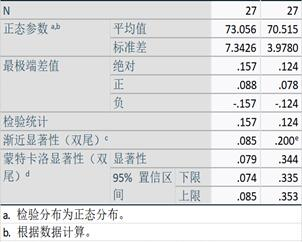
\includegraphics[width=0.45\textwidth]{img/1/red_k_S.png} % 图片相对位置 
	\caption{聚类汇总图} % 图片标题 
	\label{fig:figure 1} % 图片标签
\end{figure}

\begin{figure}[H]\centering
	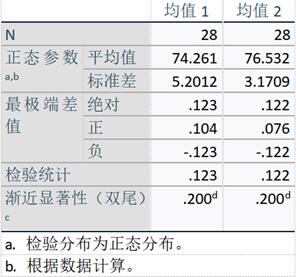
\includegraphics[width=0.45\textwidth]{img/1/white_k_S.png} % 图片相对位置 
	\caption{聚类汇总图} % 图片标题 
	\label{fig:figure 2} % 图片标签
\end{figure}

从图1\label{figure 1}和图2\label{figure 2}可以看出两组的双边检验结果。因此可以认为品酒员对葡萄酒的评分服从正态分布。

\subsubsection{两组评价结果的显著性差异评价}
上述检验显示各类葡萄酒得分情况属于正态总体,为了进一步说明品酒员评分的科学性以及两个评分组评分的可信度, 需要检查两组给出的评分是否有显著性差异, 即对数据进行显著性检验。

两配对样本非参数检验一般用于同一研究对象分别给予两种不同处理的效果比较。因为两组品酒员分别对同一样本组进行评分,故两组数据为配对数据。

\begin{equation}
	z_{li} = w_{li}-w_{2i}(i=1,2,,,,n)
\end{equation}

$z_li$来自正态分布,用假设检验的方法,假设$H_{0}:u_1=0$成立;
\[\left\{\begin{array}{llcl}

		\bar{z}=\frac{1}{n}\sum_{i=1}^n(Z_li)         \\

		s_{1}^2=\frac{1}{n-1}\sum_{i=1}^n(z_li-z_1)^2 \\

		t=\frac{\bar{z_1}}{\frac{s_1}{\sqrt{n}}}      \\

		w={\mid t \mid \ge t_{1-\frac{a}{2}}(n-1)}    \\

		% 	% S(t_0)&=&140005\times10^4&\text{人},\\
		% 	% I(t_0)&=&14052 &\text{人},\\
		% 	% R(t_0)&=&130 &\text{人},\\
		% 	% Y(t_0)&=&4562 &\text{人},\\
		% 	% N(t_0)&=&6336 &\text{人},\\
	\end{array} \right.\]

对于统计量t,在给定显著性水平a下,该检验问题的拒绝域是w,若${\mid t \mid \ge t_{1-\frac{a}{2}}(n-1)}$,则拒绝假设反之则接受。

\begin{center}
	\begin{tabular}{||c c c c c c||}
		\hline
		组数 & 样本数 & 平均值 & 标准差 & $T_1$值 & p      \\ [0.5ex]
		\hline
		一   & 27     & 73.056 & 3.9780 & 2.458   & 0.0104 \\
		\hline
		二   & 27     & 70.515 & 7.3426 & 2.458   & 0.0104 \\
		\hline
	\end{tabular}
\end{center}

上表给出了两组红葡萄酒评分均值的t检验结果,通过查表当x =0.05, n=27时, $t_{1-\frac{a}{2}}(n-1)=2.0555<2.491$
且方差齐性检验的$p$值为0.0104<0.05,
所以拒绝原假设,对于红葡萄酒的评价,两组评酒员的评价结果有显著性差异。
因为第二组评酒员对红葡萄酒样品评分的标准差大于第一组的,第二组各评酒员得评分差异小,稳定性高,比较可信。

对于白葡萄酒采用同样的方法,得到了如下的表格:
\begin{center}
	\begin{tabular}{||c c c c c c||}
		\hline
		组数 & 样本数 & 平均值 & 标准差 & $T_1$值 & p       \\ [0.5ex]
		\hline
		一   & 28     & 74.261 & 5.2012 & -2.184  & 0.01892 \\
		\hline
		二   & 28     & 76.532 & 3.1709 & -2.184  & 0.01892 \\
		\hline
	\end{tabular}
\end{center}

上表给出了两组红葡萄酒评分均值的$t$检验结果,通过查表当$x=0.05$, $n=28$时, $t_{1-\frac{a}{2}}(n-1)=2.0555<2.491$且方差齐性检验的$p$值为0. 01892<0.05,所以拒绝原假设,对于白葡萄酒的评价,两组评酒员的评价结果有显著性差异。因为第一组评酒员对红葡萄酒样品评分的标准差大于第二组,第二组各评酒员得评分差异小,稳定性高,比较可信。

综上分别对两组葡萄酒进行T检验\cite{de2013using},在显著性水平为0.05时,得出两组评酒员的评价结果有显著性差异,第二组评酒员的评分更可信。

\subsection{问题二的求解}
\subsubsection{模型建立}
由于没有目标等级函数,故需要使用无监督算法进行分类,通过分析无监督聚类算法的利弊,我们最终决定使用K-means++聚类后的结果作为最终聚类结果。


\begin{itemize}
	\item [1)]聚类分析法

	      聚类分析的基本原则:将每个评价指标作为一个维度,得分看做该特征在该维度上的坐标。通过特征向量计算数据在高纬上的距离,距离越近则认为越相近。把相似程度较大的样品聚合为一类,另一些相似程度较大的样品聚合为另一类,关系密切的聚合到一个小的分类单位,关系疏远的聚合到一个大的分类单位,直到把所有样品聚合完毕。
	      \begin{itemize}
		      \item [(1)]首先将样本中的n个点各看作一类,此时共有n类。
		      \item [(2)]计算类与类之间的距离,并将距离最短的两类合并成为一个新类。
		      \item [(3)]再重新计算类与类之间的距离,并将并将距离最短的两类合并成为一个新类。如此不断重复,直到所有的样品合为一类。
	      \end{itemize}
	\item [2)]数据处理

	      为了降低计算量,我们计划使用IPCA\cite{jeong2009ipca}代替PCA\cite{daffertshofer2004pca}将评价得分进行降维。

	      \begin{table*}[h!]
		      \begin{center}
			      \caption{KMO检验和Bartlett的检验}
			      \begin{tabular}{c c c}
				      \hline
				      KMO值                                                    & 0.000             \\
				      \hline
				      \multicolumn{1}{c|}{\multirow{3}{*}{Bartlett球形度检验}} & 近似卡方 & 0.000  \\
				      \multicolumn{1}{c|}{}                                    & df       & 55.000 \\
				      \multicolumn{1}{c|}{}                                    & p        & NaN    \\
				      \hline
			      \end{tabular}
		      \end{center}
	      \end{table*}
	      KMO检验\cite{dziuban1974correlation}的结果显示,KMO的值为NaN,同时,Bartlett球形检验的结果显示,显著性P值为NaN,水平上不呈现显著性,接受原假设,也就是变量间彼此独立,则无法从中提取公因子,主成分分析无效,建议调整数据质量,程度为极不适合。故此,我们放弃降维的做法,采用计算10个品酒师评分的均值作为特征值,而不是将10个品酒师的评价都作为特征。

	      为了消除评分的主观性,得到一个更客观的评价结果,避免出现葡萄酒因为品酒师的个人喜恶等多种因素造成评分与实践的不匹配结果,$M_{kl}$为第$k$个酒样品的第$l$个项目的十个评分,$x_{kl_{max}}$为$M_{kl}$中的最大值,$x_{kl_{min}}$为最小值。故,处理后的$M_{kl_{new}}$有:

	      \begin{equation}
		      M_{kl_{new}}=\{x_{kli}| x_{kli} ∈ M_{kl} , x_{kli}\neq x_{kl_{max}}, x_{kli} \neq x_{kl_{min}}\}
	      \end{equation}

	      为了克服由于指标的纲量不同对统计分析结果带来的影响需要对原始数据进行标准化处理,以消除单位、数据大小不一致等的影响,我们进行数据特征处理。$x_i$为去除最大最小值后的数据,$\hat{x_i}$为第i个指标的均值,$S_i$为第i个指标的标准差,$x^*_{ij}$为标准化处理以后的指标值,则有:

	      \begin{equation}
		      x^*_{ij}=\frac{x_i-\hat{x_i}}{S_i}
	      \end{equation}

\end{itemize}

\subsubsection{模型求解}
Robert Parker独一无二的葡萄酒评分体系已经成为一款新酒能否畅销的命运指挥棒。我们学习Robert Parker品酒体系使用K-means聚类算法,根据每个人的评分结果将酒样自动聚为6类。

但是,传统的K-means算法至少有两个主要的理论缺陷:
\begin{itemize}
	\item 已经证明该算法的最坏情况运行时间是输入大小的超多项式\cite{arthur2006slow}。
	\item 与最优聚类相比,所发现的近似值相对于目标函数可能是任意差的。
\end{itemize}

故此,我们使用改进后的K-means++ 算法,该算法通过在继续进行标准 K-means优化迭代之前指定初始化聚类中心的过程来解决这些障碍中的第二个障碍。通过 K-means++ 初始化,该算法可以保证找到一个与最优 K-means解具有竞争力的$ O(log k)$解。

\begin{itemize}
	\item [1)] K-mean++聚类算法
	      直观上进行解释,就是分散出k个初始聚类中心:从正在聚类的数据点中随机选择第一个聚类中心,然后从剩余的数据点中选择每个后续聚类中心,其概率与其与点最近的现有聚类中心的平方距离成正比。
	      \begin{algorithm}[htb]
		      \caption{ K-means++ 算法流程图}
		      \label{alg:Framwork}
		      \begin{algorithmic}[1]
			      \Require
			      \State 在数据点中随机选择一个中心;
			      \State 设置聚类个数K;
			      \Ensure
			      % 	Ensemble of classifiers on the current batch, $E_n$;
			      \State 对于尚未选择的每个数据点 x,计算 D(x),即 x 与已选择的最近中心之间的距离;
			      %   \label{code:fram:extract}
			      \State 使用加权概率分布随机选择一个新数据点作为新中心,其中选择概率与 D(x)2 成正比的点 x;
			      %   \label{code:fram:trainbase}
			      \State 重复步骤 2 和 3,直到选择了 k 个中心;
			      %   \label{code:fram:add}
			      \State 已选择初始中心,继续使用标准 K-means聚类;
			      %   \label{code:fram:classify}
			      %   \State Deleting some weak classifiers in $E_n$ so as to keep the capacity of $E_n$;
			      %   \label{code:fram:select} \\
			      \Return 聚类结果;
		      \end{algorithmic}
	      \end{algorithm}
	      这种播种方法显著改善了 K-means的最终误差。虽然算法中的初始选择需要额外的时间,但 K-means部分本身在此种子设定后收敛得非常快,因此算法实际上降低了计算时间。作者使用真实和合成数据集测试了他们的方法,并且通常获得了2倍的速度提高,对于某些数据集,误差提高了近1000倍。在这些模拟中,新方法在速度和误差方面几乎总是至少与普通k均值一样好。

	      此外,作者为他们的算法计算了近似比。K-means++ 算法保证期望值中的近似比 $O(log k)$(在算法的随机性上),其中k是使用的聚类数。这与普通 K-means相反,后者可以生成任意比最优值更差的聚类\cite{kanungo2004local}。 K-means++ 在相对于任意距离中具有更好的表现性能。

	\item [2)] 数据处理结果展示

	      使用SPSS软件以及Python进行数据处理,下面展示处理后的部分数据。

	      \begin{table}[!ht]
		      \centering
		      \caption{数据处理结果展示}
		      \resizebox{\textwidth}{55mm}{
			      \resizebox{\textheight}{650mm}{
				      \begin{tabular}{|c|c|c|c|c|c|c|c|c|c|c|c|}
					      \hline
					      酒样品 & 香气浓度     & 口感浓度    & 澄清度       & 香气纯正度   & 总和         & 香气质量     & 平衡/整体评价 & 口感质量     & 色调         & 口感纯正度   & 口感持久性   \\ \hline
					      1      & -0.004004004 & 0.004967384 & 0.001187377  & -0.005895169 & -0.000776987 & -0.004585114 & -0.00224002   & -0.003752651 & 0.016635279  & -0.000777495 & 0.002962963  \\ \hline
					      2      & -0.001001001 & 0.007178144 & -4.56684E-05 & 0.006215558  & 0.000767127  & -0.00698896  & 0.000245482   & 0.002121064  & 0.005335844  & 0.001130902  & 0.002962963  \\ \hline
					      3      & 0.005005005  & 0.007178144 & -4.56684E-05 & 0.006215558  & 0.003429392  & 0.005030271  & 0.000245482   & 0.002121064  & 0.005335844  & 0.001130902  & 0.002962963  \\ \hline
					      4      & -0.001001001 & -0.00756025 & -4.56684E-05 & 0.006215558  & 0.000234674  & -0.000979345 & 0.000245482   & 0.002121064  & 0.005335844  & 0.001130902  & -0.003703704 \\ \hline
					      5      & -0.013013013 & -0.00756025 & -4.56684E-05 & -0.002434961 & -0.000830232 & -0.000979345 & 0.000245482   & 0.002121064  & 0.005335844  & 0.001130902  & 0.002962963  \\ \hline
					      6      & -0.001001001 & -0.00756025 & -4.56684E-05 & -0.002434961 & -0.001362685 & -0.000979345 & 0.000245482   & 0.002121064  & -0.008788449 & 0.001130902  & -0.003703704 \\ \hline
					      7      & -0.001001001 & 0.007178144 & -4.56684E-05 & -0.01108548  & -0.001362685 & -0.000979345 & 0.000245482   & 0.002121064  & -0.022912743 & 0.001130902  & 0.002962963  \\ \hline
					      8      & -0.013013013 & -0.00756025 & -4.56684E-05 & -0.01108548  & -0.005622309 & -0.00698896  & -0.00389702   & -0.00522108  & 0.005335844  & -0.008411083 & -0.003703704 \\ \hline
					      9      & 0.005005005  & -0.00756025 & -4.56684E-05 & 0.006215558  & 0.001832033  & 0.005030271  & 0.000245482   & 0.002121064  & 0.005335844  & 0.001130902  & -0.003703704 \\ \hline
					      10     & -0.001001001 & 0.007178144 & -4.56684E-05 & 0.006215558  & 0.00129958   & -0.000979345 & 0.000245482   & 0.002121064  & 0.005335844  & 0.001130902  & -0.003703704 \\ \hline
					      11     & 0.005005005  & 0.007178144 & -4.56684E-05 & -0.01108548  & -0.002960044 & -0.000979345 & 0.000245482   & -0.00522108  & -0.022912743 & -0.008411083 & 0.002962963  \\ \hline
					      12     & 0.005005005  & 0.007178144 & -4.56684E-05 & -0.002434961 & 0.000767127  & 0.005030271  & 0.000245482   & 0.002121064  & -0.022912743 & 0.001130902  & 0.002962963  \\ \hline
					      13     & -0.001001001 & -0.00756025 & -4.56684E-05 & 0.006215558  & -0.002427591 & -0.000979345 & 0.000245482   & -0.00522108  & -0.008788449 & 0.001130902  & -0.003703704 \\ \hline
					      14     & -0.001001001 & 0.007178144 & -4.56684E-05 & -0.002434961 & 0.00129958   & -0.000979345 & 0.000245482   & 0.002121064  & 0.005335844  & 0.001130902  & 0.002962963  \\ \hline
					      15     & -0.001001001 & 0.007178144 & -4.56684E-05 & -0.01108548  & -0.000297779 & -0.00698896  & 0.000245482   & 0.002121064  & 0.005335844  & 0.001130902  & 0.002962963  \\ \hline
					      16     & -0.001001001 & -0.00756025 & -4.56684E-05 & -0.01108548  & -0.000297779 & -0.000979345 & 0.000245482   & 0.002121064  & 0.005335844  & 0.001130902  & 0.002962963  \\ \hline
					      17     & -0.001001001 & 0.007178144 & -4.56684E-05 & -0.002434961 & -0.000830232 & -0.000979345 & 0.000245482   & -0.00522108  & 0.005335844  & 0.001130902  & -0.003703704 \\ \hline
					      18     & -0.001001001 & 0.007178144 & -4.56684E-05 & -0.01108548  & -0.002427591 & -0.00698896  & 0.000245482   & 0.002121064  & -0.022912743 & 0.001130902  & 0.002962963  \\ \hline
					      19     & -0.001001001 & -0.00756025 & -4.56684E-05 & 0.006215558  & 0.000767127  & -0.000979345 & 0.000245482   & 0.002121064  & 0.005335844  & 0.001130902  & 0.002962963  \\ \hline
					      20     & 0.005005005  & -0.00756025 & -4.56684E-05 & 0.006215558  & 0.000234674  & 0.005030271  & 0.000245482   & 0.002121064  & -0.022912743 & 0.001130902  & 0.002962963  \\ \hline
					      21     & 0.005005005  & 0.007178144 & -4.56684E-05 & 0.006215558  & 0.004494298  & 0.005030271  & 0.000245482   & 0.002121064  & 0.019460138  & 0.001130902  & 0.002962963  \\ \hline
					      22     & 0.005005005  & -0.00756025 & -4.56684E-05 & 0.006215558  & 0.001832033  & 0.005030271  & 0.000245482   & 0.002121064  & 0.005335844  & 0.001130902  & -0.003703704 \\ \hline
					      23     & 0.005005005  & 0.007178144 & -4.56684E-05 & 0.006215558  & 0.002364486  & 0.011039886  & 0.000245482   & -0.00522108  & 0.005335844  & 0.001130902  & -0.003703704 \\ \hline
					      24     & 0.005005005  & -0.00756025 & -4.56684E-05 & 0.006215558  & 0.000234674  & 0.005030271  & 0.000245482   & -0.00522108  & 0.005335844  & 0.001130902  & -0.003703704 \\ \hline
					      25     & -0.001001001 & -0.00756025 & -4.56684E-05 & 0.006215558  & -0.001895138 & -0.000979345 & 0.000245482   & -0.00522108  & 0.005335844  & -0.008411083 & -0.003703704 \\ \hline
					      26     & -0.001001001 & 0.007178144 & -4.56684E-05 & 0.006215558  & 0.001832033  & -0.000979345 & 0.000245482   & 0.002121064  & 0.005335844  & 0.001130902  & 0.002962963  \\ \hline
					      27     & -0.001001001 & -0.00756025 & -4.56684E-05 & -0.002434961 & -0.000297779 & -0.000979345 & 0.000245482   & 0.002121064  & 0.005335844  & 0.001130902  & -0.003703704 \\ \hline
				      \end{tabular}}}
	      \end{table}



	\item [3)] 问题求解

	      \begin{itemize}
		      \item [A]分析步骤
		            \begin{itemize}
			            \item 根据字段进行聚类类别差异性分析;
			            \item 根据聚类汇总分析各聚类类别的频数;
			            \item 根据数据集聚类标注可以知道每一个样本数据被分到哪个类别;
			            \item 聚类中心坐标可以用于分析各样本与中心点的距离;
			            \item 对分析进行综述。
		            \end{itemize}
		      \item [B]聚类分析结果

		            下表展示了定量字段差异性分析的结果,包括均值±标准差的结果、F检验结果、显著性P值。
		            \begin{itemize}
			            \item 分析每个分析项是否小于0.05或者0.01(根据检验标准要求,严格的话使用0.01);
			            \item 若呈显著性,拒绝原假设,说明两组数据之间存在显著性差异,可以根据均值±标准差的方式对差异进行分析,反之则表明数据不呈现差异性。
		            \end{itemize}

		            方差分析的结果显示:
		            对于变量澄清度,显著性P值为0.911,水平上不呈现显著性,不能拒绝原假设,说明变量澄清度在聚类分析划分的类别之间不存在显著性差异;

		            对于变量色调,显著性P值为0.000***,水平上呈现显著性,拒绝原假设,说明变量色调2在聚类分析划分的类别之间存在显著性差异;

		            对于变量香气浓度,显著性P值为0.001***,水平上呈现显著性,拒绝原假设,说明变量香气浓度2在聚类分析划分的类别之间存在显著性差异;

		            对于变量口感浓度,显著性P值为0.522,水平上不呈现显著性,不能拒绝原假设,说明变量口感浓度2在聚类分析划分的类别之间不存在显著性差异;

		            对于变量香气纯正度,显著性P值为0.014**,水平上呈现显著性,拒绝原假设,说明变量香气纯正度2在聚类分析划分的类别之间存在显著性差异;

		            对于变量口感持久性,显著性P值为0.316,水平上不呈现显著性,不能拒绝原假设,说明变量口感持久性2在聚类分析划分的类别之间不存在显著性差异;

		            对于变量口感质量,显著性P值为0.445,水平上不呈现显著性,不能拒绝原假设,说明变量口感质量2在聚类分析划分的类别之间不存在显著性差异;

		            对于变量香气质量,显著性P值为0.002***,水平上呈现显著性,拒绝原假设,说明变量香气质量2在聚类分析划分的类别之间存在显著性差异;

		            对于变量平衡/整体评价,显著性P值为0.000***,水平上呈现显著性,拒绝原假设,说明变量平衡/整体评价2在聚类分析划分的类别之间存在显著性差异;

		            对于变量口感纯正度,显著性P值为0.056*,水平上不呈现显著性,不能拒绝原假设,说明变量口感纯正度2在聚类分析划分的类别之间不存在显著性差异;

		            对于变量总和,显著性P值为0.000***,水平上呈现显著性,拒绝原假设,说明变量总和在聚类分析划分的类别之间存在显著性差异;
		            \begin{table}[!ht]
			            \centering

			            \caption{字段差异性分析(***、**、*分别代表1\%、5\%、10\%的显著性水平)}
			            \resizebox{\textwidth}{30mm}{
				            \resizebox{\textheight}{60mm}{
					            \begin{tabular}{|c|c|c|c|c|c|c|c|c|}
						            \hline
						            \multicolumn{7}{|c|}{聚类类别(平均值 ± 标准差} & F           & P                                                                                              \\\hline
						            ~                                               & 类别2(n=6)  & 类别3(n=6)   & 类别5(n=4)   & 类别6(n=4)   & 类别4(n=4)   & 类别1(n=3)   & ~        & ~        \\ \hline
						            澄清度                                          & -0.0±0.0    & -0.0±0.0     & 0.0±0.001    & -0.0±0.0     & -0.0±0.0     & -0.0±0.0     & 1.193    & 0.346    \\ \hline
						            香气纯正度                                      & 0.006±0.0   & 0.006±0.0    & -0.005±0.004 & -0.007±0.005 & -0.009±0.004 & 0.003±0.005  & 20.321   & 0.000*** \\ \hline
						            香气浓度                                        & 0.002±0.003 & 0.002±0.003  & -0.002±0.002 & -0.007±0.007 & 0.002±0.003  & 0.001±0.003  & 3.627    & 0.016**  \\ \hline
						            平衡/整体评价                                   & 0.0±0.0     & 0.0±0.0      & -0.0±0.001   & -0.001±0.002 & 0.0±0.0      & 0.0±0.0      & 1.01     & 0.437    \\ \hline
						            总和                                            & 0.002±0.001 & 0.001±0.001  & -0.0±0.001   & -0.002±0.003 & -0.001±0.002 & -0.001±0.001 & 4.73     & 0.005*** \\ \hline
						            香气质量                                        & 0.002±0.006 & 0.002±0.003  & -0.003±0.003 & -0.002±0.003 & -0.001±0.005 & 0.001±0.003  & 1.322    & 0.293    \\ \hline
						            口感质量                                        & 0.001±0.003 & -0.0±0.004   & -0.001±0.004 & 0.0±0.004    & 0.0±0.004    & -0.0±0.004   & 0.182    & 0.966    \\ \hline
						            口感浓度                                        & 0.007±0.0   & -0.008±0.0   & 0.007±0.001  & -0.008±0.0   & 0.007±0.0    & -0.008±0.0   & 1642.937 & 0.000*** \\ \hline
						            色调                                            & 0.008±0.006 & 0.005±0.0    & 0.008±0.006  & 0.005±0.0    & -0.023±0.0   & -0.013±0.008 & 37.772   & 0.000*** \\ \hline
						            口感纯正度                                      & 0.001±0.0   & -0.0±0.004   & 0.001±0.001  & -0.001±0.005 & -0.001±0.005 & 0.001±0.0    & 0.529    & 0.752    \\ \hline
						            口感持久性                                      & 0.001±0.003 & -0.003±0.003 & 0.001±0.003  & -0.0±0.004   & 0.003±0.0    & -0.001±0.004 & 1.909    & 0.136    \\ \hline
					            \end{tabular}}}
		            \end{table}


		            下表展示了模型聚类的结果,包括频数,所占百分比。
		            聚类分析的结果显示,聚类结果共分为6类,不同聚类类别对应频数和百分比如下表,并可视化展示模型聚类的结果,包括频数,所占百分比。

		            \begin{table}[!ht]
			            \centering
			            \caption{聚类汇总}
			            \begin{tabular}{|c|c|c|}
				            \hline
				            聚类类别  & 频数 & 百分比\% \\ \hline
				            聚类类别1 & 3    & 11.111\% \\ \hline
				            聚类类别2 & 6    & 22.222\% \\ \hline
				            聚类类别3 & 6    & 22.222\% \\ \hline
				            聚类类别4 & 4    & 14.815\% \\ \hline
				            聚类类别5 & 4    & 14.815\% \\ \hline
				            聚类类别6 & 4    & 14.815\% \\ \hline
				            合计      & 27   & 100.0\%  \\ \hline
			            \end{tabular}
		            \end{table}


		            \begin{figure}[H]\centering
			            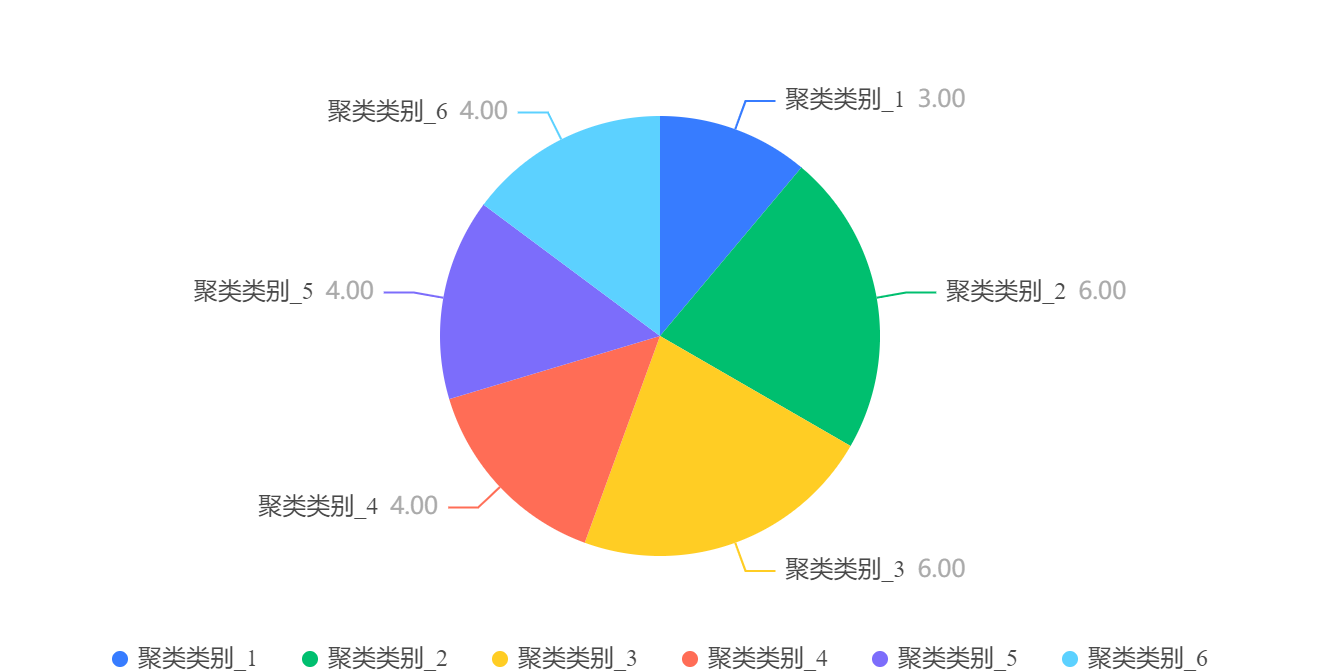
\includegraphics[width=0.9\textwidth]{img/2/Cluster_summary.png} % 图片相对位置 
			            \caption{聚类汇总图} % 图片标题 
			            \label{fig:figure 10} % 图片标签
		            \end{figure}

		            上表格展示了模型聚类结果的部分数据聚类标注,其为预览结果,只显示综合排序的前10条数。

		            \begin{table}[!ht]
			            \centering
			            \caption{数据集聚类标注}
			            \resizebox{\textwidth}{50mm}{
				            \resizebox{\textheight}{250mm}{
					            \begin{tabular}{|c|c|c|c|c|c|c|c|c|c|c|c|}
						            \hline
						            聚类种类 & 澄清度      & 香气纯正度   & 香气浓度     & 平衡/整体评价 & 总和         & 香气质量     & 口感质量     & 口感浓度    & 色调         & 口感纯正度   & 口感持久性   \\ \hline
						            5        & 0.001187377 & -0.005895169 & -0.004004004 & -0.00224002   & -0.000776987 & -0.004585114 & -0.003752651 & 0.004967384 & 0.016635279  & -0.000777495 & 0.002962963  \\ \hline
						            2        & -4.57E-05   & 0.006215558  & -0.001001001 & 0.000245482   & 0.000767127  & -0.00698896  & 0.002121064  & 0.007178144 & 0.005335844  & 0.001130902  & 0.002962963  \\ \hline
						            2        & -4.57E-05   & 0.006215558  & 0.005005005  & 0.000245482   & 0.003429392  & 0.005030271  & 0.002121064  & 0.007178144 & 0.005335844  & 0.001130902  & 0.002962963  \\ \hline
						            3        & -4.57E-05   & 0.006215558  & -0.001001001 & 0.000245482   & 0.000234674  & -0.000979345 & 0.002121064  & -0.00756025 & 0.005335844  & 0.001130902  & -0.003703704 \\ \hline
						            6        & -4.57E-05   & -0.002434961 & -0.013013013 & 0.000245482   & -0.000830232 & -0.000979345 & 0.002121064  & -0.00756025 & 0.005335844  & 0.001130902  & 0.002962963  \\ \hline
						            1        & -4.57E-05   & -0.002434961 & -0.001001001 & 0.000245482   & -0.001362685 & -0.000979345 & 0.002121064  & -0.00756025 & -0.008788449 & 0.001130902  & -0.003703704 \\ \hline
						            4        & -4.57E-05   & -0.01108548  & -0.001001001 & 0.000245482   & -0.001362685 & -0.000979345 & 0.002121064  & 0.007178144 & -0.022912743 & 0.001130902  & 0.002962963  \\ \hline
						            6        & -4.57E-05   & -0.01108548  & -0.013013013 & -0.00389702   & -0.005622309 & -0.00698896  & -0.00522108  & -0.00756025 & 0.005335844  & -0.008411083 & -0.003703704 \\ \hline
						            3        & -4.57E-05   & 0.006215558  & 0.005005005  & 0.000245482   & 0.001832033  & 0.005030271  & 0.002121064  & -0.00756025 & 0.005335844  & 0.001130902  & -0.003703704 \\ \hline
						            2        & -4.57E-05   & 0.006215558  & -0.001001001 & 0.000245482   & 0.00129958   & -0.000979345 & 0.002121064  & 0.007178144 & 0.005335844  & 0.001130902  & -0.003703704 \\ \hline
						            4        & -4.57E-05   & -0.01108548  & 0.005005005  & 0.000245482   & -0.002960044 & -0.000979345 & -0.00522108  & 0.007178144 & -0.022912743 & -0.008411083 & 0.002962963  \\ \hline
						            4        & -4.57E-05   & -0.002434961 & 0.005005005  & 0.000245482   & 0.000767127  & 0.005030271  & 0.002121064  & 0.007178144 & -0.022912743 & 0.001130902  & 0.002962963  \\ \hline
						            1        & -4.57E-05   & 0.006215558  & -0.001001001 & 0.000245482   & -0.002427591 & -0.000979345 & -0.00522108  & -0.00756025 & -0.008788449 & 0.001130902  & -0.003703704 \\ \hline
						            5        & -4.57E-05   & -0.002434961 & -0.001001001 & 0.000245482   & 0.00129958   & -0.000979345 & 0.002121064  & 0.007178144 & 0.005335844  & 0.001130902  & 0.002962963  \\ \hline
						            5        & -4.57E-05   & -0.01108548  & -0.001001001 & 0.000245482   & -0.000297779 & -0.00698896  & 0.002121064  & 0.007178144 & 0.005335844  & 0.001130902  & 0.002962963  \\ \hline
						            6        & -4.57E-05   & -0.01108548  & -0.001001001 & 0.000245482   & -0.000297779 & -0.000979345 & 0.002121064  & -0.00756025 & 0.005335844  & 0.001130902  & 0.002962963  \\ \hline
						            5        & -4.57E-05   & -0.002434961 & -0.001001001 & 0.000245482   & -0.000830232 & -0.000979345 & -0.00522108  & 0.007178144 & 0.005335844  & 0.001130902  & -0.003703704 \\ \hline
						            4        & -4.57E-05   & -0.01108548  & -0.001001001 & 0.000245482   & -0.002427591 & -0.00698896  & 0.002121064  & 0.007178144 & -0.022912743 & 0.001130902  & 0.002962963  \\ \hline
						            3        & -4.57E-05   & 0.006215558  & -0.001001001 & 0.000245482   & 0.000767127  & -0.000979345 & 0.002121064  & -0.00756025 & 0.005335844  & 0.001130902  & 0.002962963  \\ \hline
						            1        & -4.57E-05   & 0.006215558  & 0.005005005  & 0.000245482   & 0.000234674  & 0.005030271  & 0.002121064  & -0.00756025 & -0.022912743 & 0.001130902  & 0.002962963  \\ \hline
						            2        & -4.57E-05   & 0.006215558  & 0.005005005  & 0.000245482   & 0.004494298  & 0.005030271  & 0.002121064  & 0.007178144 & 0.019460138  & 0.001130902  & 0.002962963  \\ \hline
						            3        & -4.57E-05   & 0.006215558  & 0.005005005  & 0.000245482   & 0.001832033  & 0.005030271  & 0.002121064  & -0.00756025 & 0.005335844  & 0.001130902  & -0.003703704 \\ \hline
						            2        & -4.57E-05   & 0.006215558  & 0.005005005  & 0.000245482   & 0.002364486  & 0.011039886  & -0.00522108  & 0.007178144 & 0.005335844  & 0.001130902  & -0.003703704 \\ \hline
						            3        & -4.57E-05   & 0.006215558  & 0.005005005  & 0.000245482   & 0.000234674  & 0.005030271  & -0.00522108  & -0.00756025 & 0.005335844  & 0.001130902  & -0.003703704 \\ \hline
						            3        & -4.57E-05   & 0.006215558  & -0.001001001 & 0.000245482   & -0.001895138 & -0.000979345 & -0.00522108  & -0.00756025 & 0.005335844  & -0.008411083 & -0.003703704 \\ \hline
						            2        & -4.57E-05   & 0.006215558  & -0.001001001 & 0.000245482   & 0.001832033  & -0.000979345 & 0.002121064  & 0.007178144 & 0.005335844  & 0.001130902  & 0.002962963  \\ \hline
						            6        & -4.57E-05   & -0.002434961 & -0.001001001 & 0.000245482   & -0.000297779 & -0.000979345 & 0.002121064  & -0.00756025 & 0.005335844  & 0.001130902  & -0.003703704 \\ \hline
					            \end{tabular}}}
		            \end{table}

		            \begin{table}[!ht]
			            \centering
			            \caption{聚类中心点坐标}
			            \resizebox{\textwidth}{13mm}{
				            \resizebox{\textheight}{10mm}{
					            \begin{tabular}{|c|c|c|c|c|c|c|c|c|c|c|c|}
						            \hline
						            聚类种类 & 澄清度      & 香气纯正度   & 香气浓度     & 平衡/整体评价 & 总和         & 香气质量     & 口感质量     & 口感浓度    & 色调         & 口感纯正度   & 口感持久性   \\ \hline
						            1        & -4.57E-05   & 0.003332052  & 0.001001001  & 0.000245482   & -0.001185201 & 0.00102386   & -0.000326318 & -0.00756025 & -0.013496547 & 0.001130902  & -0.001481481 \\ \hline
						            2        & -4.57E-05   & 0.006215558  & 0.002002002  & 0.000245482   & 0.002364486  & 0.002025463  & 0.000897373  & 0.007178144 & 0.007689893  & 0.001130902  & 0.000740741  \\ \hline
						            3        & -4.57E-05   & 0.006215558  & 0.002002002  & 0.000245482   & 0.0005009    & 0.002025463  & -0.000326318 & -0.00756025 & 0.005335844  & -0.000459429 & -0.002592593 \\ \hline
						            4        & -4.57E-05   & -0.00892285  & 0.002002002  & 0.000245482   & -0.001495799 & -0.000979345 & 0.000285528  & 0.007178144 & -0.022912743 & -0.001254594 & 0.002962963  \\ \hline
						            5        & 0.000262593 & -0.005462643 & -0.001751752 & -0.000375894  & -0.000151355 & -0.003383191 & -0.001182901 & 0.006625454 & 0.008160703  & 0.000653803  & 0.001296296  \\ \hline
						            6        & -4.57E-05   & -0.00676022  & -0.007007007 & -0.000790144  & -0.001762025 & -0.002481749 & 0.000285528  & -0.00756025 & 0.005335844  & -0.001254594 & -0.00037037  \\ \hline
					            \end{tabular}}}
		            \end{table}

	      \end{itemize}
	\item[4] 聚类结果分析

		我们可以明显的发现,算法自动将评分接近的样本酒聚为一类,随着聚类种类编号数的上升,酒样的评分越高,聚类结果体现了我们算法的有效性。
		\begin{table}[!ht]
			\centering
			\caption{红酒聚类结果分析}
			\resizebox{\textwidth}{55mm}{
				\resizebox{\textheight}{200mm}{
					\begin{tabular}{|c|c|c|c|c|c|c|c|c|c|c|c|c|}
						\hline
						酒样本 & 聚类种类 & 澄清度 & 色调 & 香气浓度 & 口感浓度 & 香气纯正度 & 口感持久性 & 口感质量 & 香气质量 & 平衡/整体评价 & 口感纯正度 & 总和 \\ \hline
						7      & 1        & 3      & 6    & 4        & 4        & 3          & 27         & 13       & 10       & 8             & 3          & 59   \\ \hline
						0      & 2        & 3.1    & 7.6  & 5.5      & 5.7      & 3.6        & 3          & 13.6     & 10.8     & 8.4           & 3.8        & 68.1 \\ \hline
						1      & 2        & 3      & 6    & 6        & 6        & 5          & 4          & 16       & 10       & 9             & 4          & 71   \\ \hline
						3      & 2        & 3      & 6    & 6        & 4        & 5          & 5          & 16       & 12       & 9             & 4          & 70   \\ \hline
						4      & 2        & 3      & 6    & 4        & 4        & 4          & 6          & 16       & 12       & 9             & 4          & 68   \\ \hline
						5      & 2        & 3      & 4    & 6        & 4        & 4          & 7          & 16       & 12       & 9             & 4          & 67   \\ \hline
						14     & 2        & 3      & 6    & 6        & 6        & 3          & 8          & 16       & 10       & 9             & 4          & 69   \\ \hline
						15     & 2        & 3      & 6    & 6        & 4        & 3          & 9          & 16       & 12       & 9             & 4          & 69   \\ \hline
						16     & 2        & 3      & 6    & 6        & 6        & 4          & 10         & 13       & 12       & 9             & 4          & 68   \\ \hline
						24     & 2        & 3      & 6    & 6        & 4        & 5          & 11         & 13       & 12       & 9             & 3          & 66   \\ \hline
						26     & 2        & 3      & 6    & 6        & 4        & 4          & 12         & 16       & 12       & 9             & 4          & 69   \\ \hline
						8      & 3        & 3      & 6    & 7        & 4        & 5          & 13         & 16       & 14       & 9             & 4          & 73   \\ \hline
						9      & 3        & 3      & 6    & 6        & 6        & 5          & 14         & 16       & 12       & 9             & 4          & 72   \\ \hline
						13     & 3        & 3      & 6    & 6        & 6        & 4          & 15         & 16       & 12       & 9             & 4          & 72   \\ \hline
						18     & 3        & 3      & 6    & 6        & 4        & 5          & 16         & 16       & 12       & 9             & 4          & 71   \\ \hline
						21     & 3        & 3      & 6    & 7        & 4        & 5          & 17         & 16       & 14       & 9             & 4          & 73   \\ \hline
						22     & 3        & 3      & 6    & 7        & 6        & 5          & 18         & 13       & 16       & 9             & 4          & 74   \\ \hline
						23     & 3        & 3      & 6    & 7        & 4        & 5          & 19         & 13       & 14       & 9             & 4          & 70   \\ \hline
						25     & 3        & 3      & 6    & 6        & 6        & 5          & 20         & 16       & 12       & 9             & 4          & 73   \\ \hline
						6      & 4        & 3      & 2    & 6        & 6        & 3          & 21         & 16       & 12       & 9             & 4          & 67   \\ \hline
						10     & 4        & 3      & 2    & 7        & 6        & 3          & 22         & 13       & 12       & 9             & 3          & 64   \\ \hline
						12     & 4        & 3      & 4    & 6        & 4        & 5          & 23         & 13       & 12       & 9             & 4          & 65   \\ \hline
						17     & 4        & 3      & 2    & 6        & 6        & 3          & 24         & 16       & 10       & 9             & 4          & 65   \\ \hline
						11     & 5        & 3      & 2    & 7        & 6        & 4          & 25         & 16       & 14       & 9             & 4          & 71   \\ \hline
						19     & 5        & 3      & 2    & 7        & 4        & 5          & 26         & 16       & 14       & 9             & 4          & 70   \\ \hline
						2      & 6        & 3      & 6    & 7        & 6        & 5          & 28         & 16       & 14       & 9             & 4          & 76   \\ \hline
						20     & 6        & 3      & 8    & 7        & 6        & 5          & 29         & 16       & 14       & 9             & 4          & 78   \\ \hline
					\end{tabular}
				}
			}
		\end{table}

		\begin{table}[!ht]
			\centering
			\caption{白酒聚类结果分析}
			\resizebox{\textwidth}{55mm}{
				\resizebox{\textheight}{200mm}{
					\begin{tabular}{|c|c|c|c|c|c|c|c|c|c|c|c|c|}
						\hline
						酒样本 & 聚类种类 & 澄清度 & 色调 & 香气浓度 & 口感浓度 & 香气纯正度 & 口感持久性 & 口感质量 & 香气质量 & 平衡/整体评价 & 口感纯正度 & 总和 \\ \hline
						7      & 1        & 3      & 6    & 4        & 4        & 3          & 27         & 13       & 10       & 8             & 3          & 59   \\ \hline
						0      & 2        & 3.1    & 7.6  & 5.5      & 5.7      & 3.6        & 3          & 13.6     & 10.8     & 8.4           & 3.8        & 68.1 \\ \hline
						1      & 2        & 3      & 6    & 6        & 6        & 5          & 4          & 16       & 10       & 9             & 4          & 71   \\ \hline
						3      & 2        & 3      & 6    & 6        & 4        & 5          & 5          & 16       & 12       & 9             & 4          & 70   \\ \hline
						4      & 2        & 3      & 6    & 4        & 4        & 4          & 6          & 16       & 12       & 9             & 4          & 68   \\ \hline
						5      & 2        & 3      & 4    & 6        & 4        & 4          & 7          & 16       & 12       & 9             & 4          & 67   \\ \hline
						14     & 2        & 3      & 6    & 6        & 6        & 3          & 8          & 16       & 10       & 9             & 4          & 69   \\ \hline
						15     & 2        & 3      & 6    & 6        & 4        & 3          & 9          & 16       & 12       & 9             & 4          & 69   \\ \hline
						16     & 2        & 3      & 6    & 6        & 6        & 4          & 10         & 13       & 12       & 9             & 4          & 68   \\ \hline
						24     & 2        & 3      & 6    & 6        & 4        & 5          & 11         & 13       & 12       & 9             & 3          & 66   \\ \hline
						26     & 2        & 3      & 6    & 6        & 4        & 4          & 12         & 16       & 12       & 9             & 4          & 69   \\ \hline
						8      & 3        & 3      & 6    & 7        & 4        & 5          & 13         & 16       & 14       & 9             & 4          & 73   \\ \hline
						9      & 3        & 3      & 6    & 6        & 6        & 5          & 14         & 16       & 12       & 9             & 4          & 72   \\ \hline
						13     & 3        & 3      & 6    & 6        & 6        & 4          & 15         & 16       & 12       & 9             & 4          & 72   \\ \hline
						18     & 3        & 3      & 6    & 6        & 4        & 5          & 16         & 16       & 12       & 9             & 4          & 71   \\ \hline
						21     & 3        & 3      & 6    & 7        & 4        & 5          & 17         & 16       & 14       & 9             & 4          & 73   \\ \hline
						22     & 3        & 3      & 6    & 7        & 6        & 5          & 18         & 13       & 16       & 9             & 4          & 74   \\ \hline
						23     & 3        & 3      & 6    & 7        & 4        & 5          & 19         & 13       & 14       & 9             & 4          & 70   \\ \hline
						25     & 3        & 3      & 6    & 6        & 6        & 5          & 20         & 16       & 12       & 9             & 4          & 73   \\ \hline
						6      & 4        & 3      & 2    & 6        & 6        & 3          & 21         & 16       & 12       & 9             & 4          & 67   \\ \hline
						10     & 4        & 3      & 2    & 7        & 6        & 3          & 22         & 13       & 12       & 9             & 3          & 64   \\ \hline
						12     & 4        & 3      & 4    & 6        & 4        & 5          & 23         & 13       & 12       & 9             & 4          & 65   \\ \hline
						17     & 4        & 3      & 2    & 6        & 6        & 3          & 24         & 16       & 10       & 9             & 4          & 65   \\ \hline
						11     & 5        & 3      & 2    & 7        & 6        & 4          & 25         & 16       & 14       & 9             & 4          & 71   \\ \hline
						19     & 5        & 3      & 2    & 7        & 4        & 5          & 26         & 16       & 14       & 9             & 4          & 70   \\ \hline
						2      & 6        & 3      & 6    & 7        & 6        & 5          & 28         & 16       & 14       & 9             & 4          & 76   \\ \hline
						20     & 6        & 3      & 8    & 7        & 6        & 5          & 29         & 16       & 14       & 9             & 4          & 78   \\ \hline
					\end{tabular}
				}
			}
		\end{table}

\end{itemize}


\subsection{问题三的求解}
\subsubsection{数据筛选}
所给出酿酒葡萄和葡萄酒的数据十分多,但不能保证没一项指标都有一项对应的指标与他有着显著的相关性,所以需要进行数据指标的筛选,使得其相关性分析,更加可信。在本问中,抽选葡萄酒的花色苷、DPPH半抑制体积、酒总黄酮、色泽这几项数据来进行数据相关性分析。

\subsubsection{相关性分析}

相关分析是描述两个变量间关系的密切程度,由相关系数和显著性程度值表示,当相关系数的绝对值越接近于1,则表示两个变量间的相关性越显著,或者显著性*p<0.05,**p<0.01具有上述的效。双变量系数测量的主要指标有卡方类测量、Spearman相关系数、pearson相关系数等,由于酿酒葡萄和葡萄酒的数据为定距数据,则在进行两者间的相关性检验时用pearson相关系数来判断,其公式为:

\begin{equation}
	r=\frac{\sum(x_i-\bar{x})}{\sqrt{\sum(x_i-\bar{x})^2 \sum(y_i-\bar{y})^2}}
\end{equation}

相关系数r的取值范围为:$-1\le r \le 1$

\[\left\{\begin{array}{llcl}
		r>0为正相关,r<0为负相关         \\

		\mid r \mid =0表示不存在线性关系 \\

		\mid r \mid =1表示完全线性相关   \\
	\end{array} \right.\]

其中皮尔森简单相关系数检验统计为:

\begin{equation}
	t=\frac{r sqrt{n-1}}{\sqrt{1-r^2}}
\end{equation}

其中的t服从n-2个自由度的t分布

\subsubsection{相关性检验}
通过将筛选出的数据通过spss来进行相关性的检验分析,来发现针对某些特定的葡萄酒指标,有的酿酒葡萄在某个理化指标较为突出的情况下,
可以根据需求来进行指定行的处理来满足要求。如下将一次选取花色苷、DPPH半抑制体积、酒总黄酮、色泽这几项数据来进行数据相关性分析。
通过对数据进行平均值和标准差统计,成对排除个案缺失值,采用pearson相关系数的双侧显著性检验来获取结果。如下为结果图。


% 通过观察数据表的pearson相关性数据可以发现葡萄酒中花色苷的指标与褐变度、苹果酸、单宁、果梗比等数据的相关性较为显著,从而可以知道
% 该些酿酒葡萄的理化指标对花色苷的影响较为明显,同时也通过该表可以得出一些负相关的理化指标。

% 同理进行DPPH半抑制体积、酒总黄酮、色泽其余三项数据的分析,分别得出相关性分析结果

% 如图为DPPH半抑制体积的相关性分析
\begin{figure}[H]\centering
	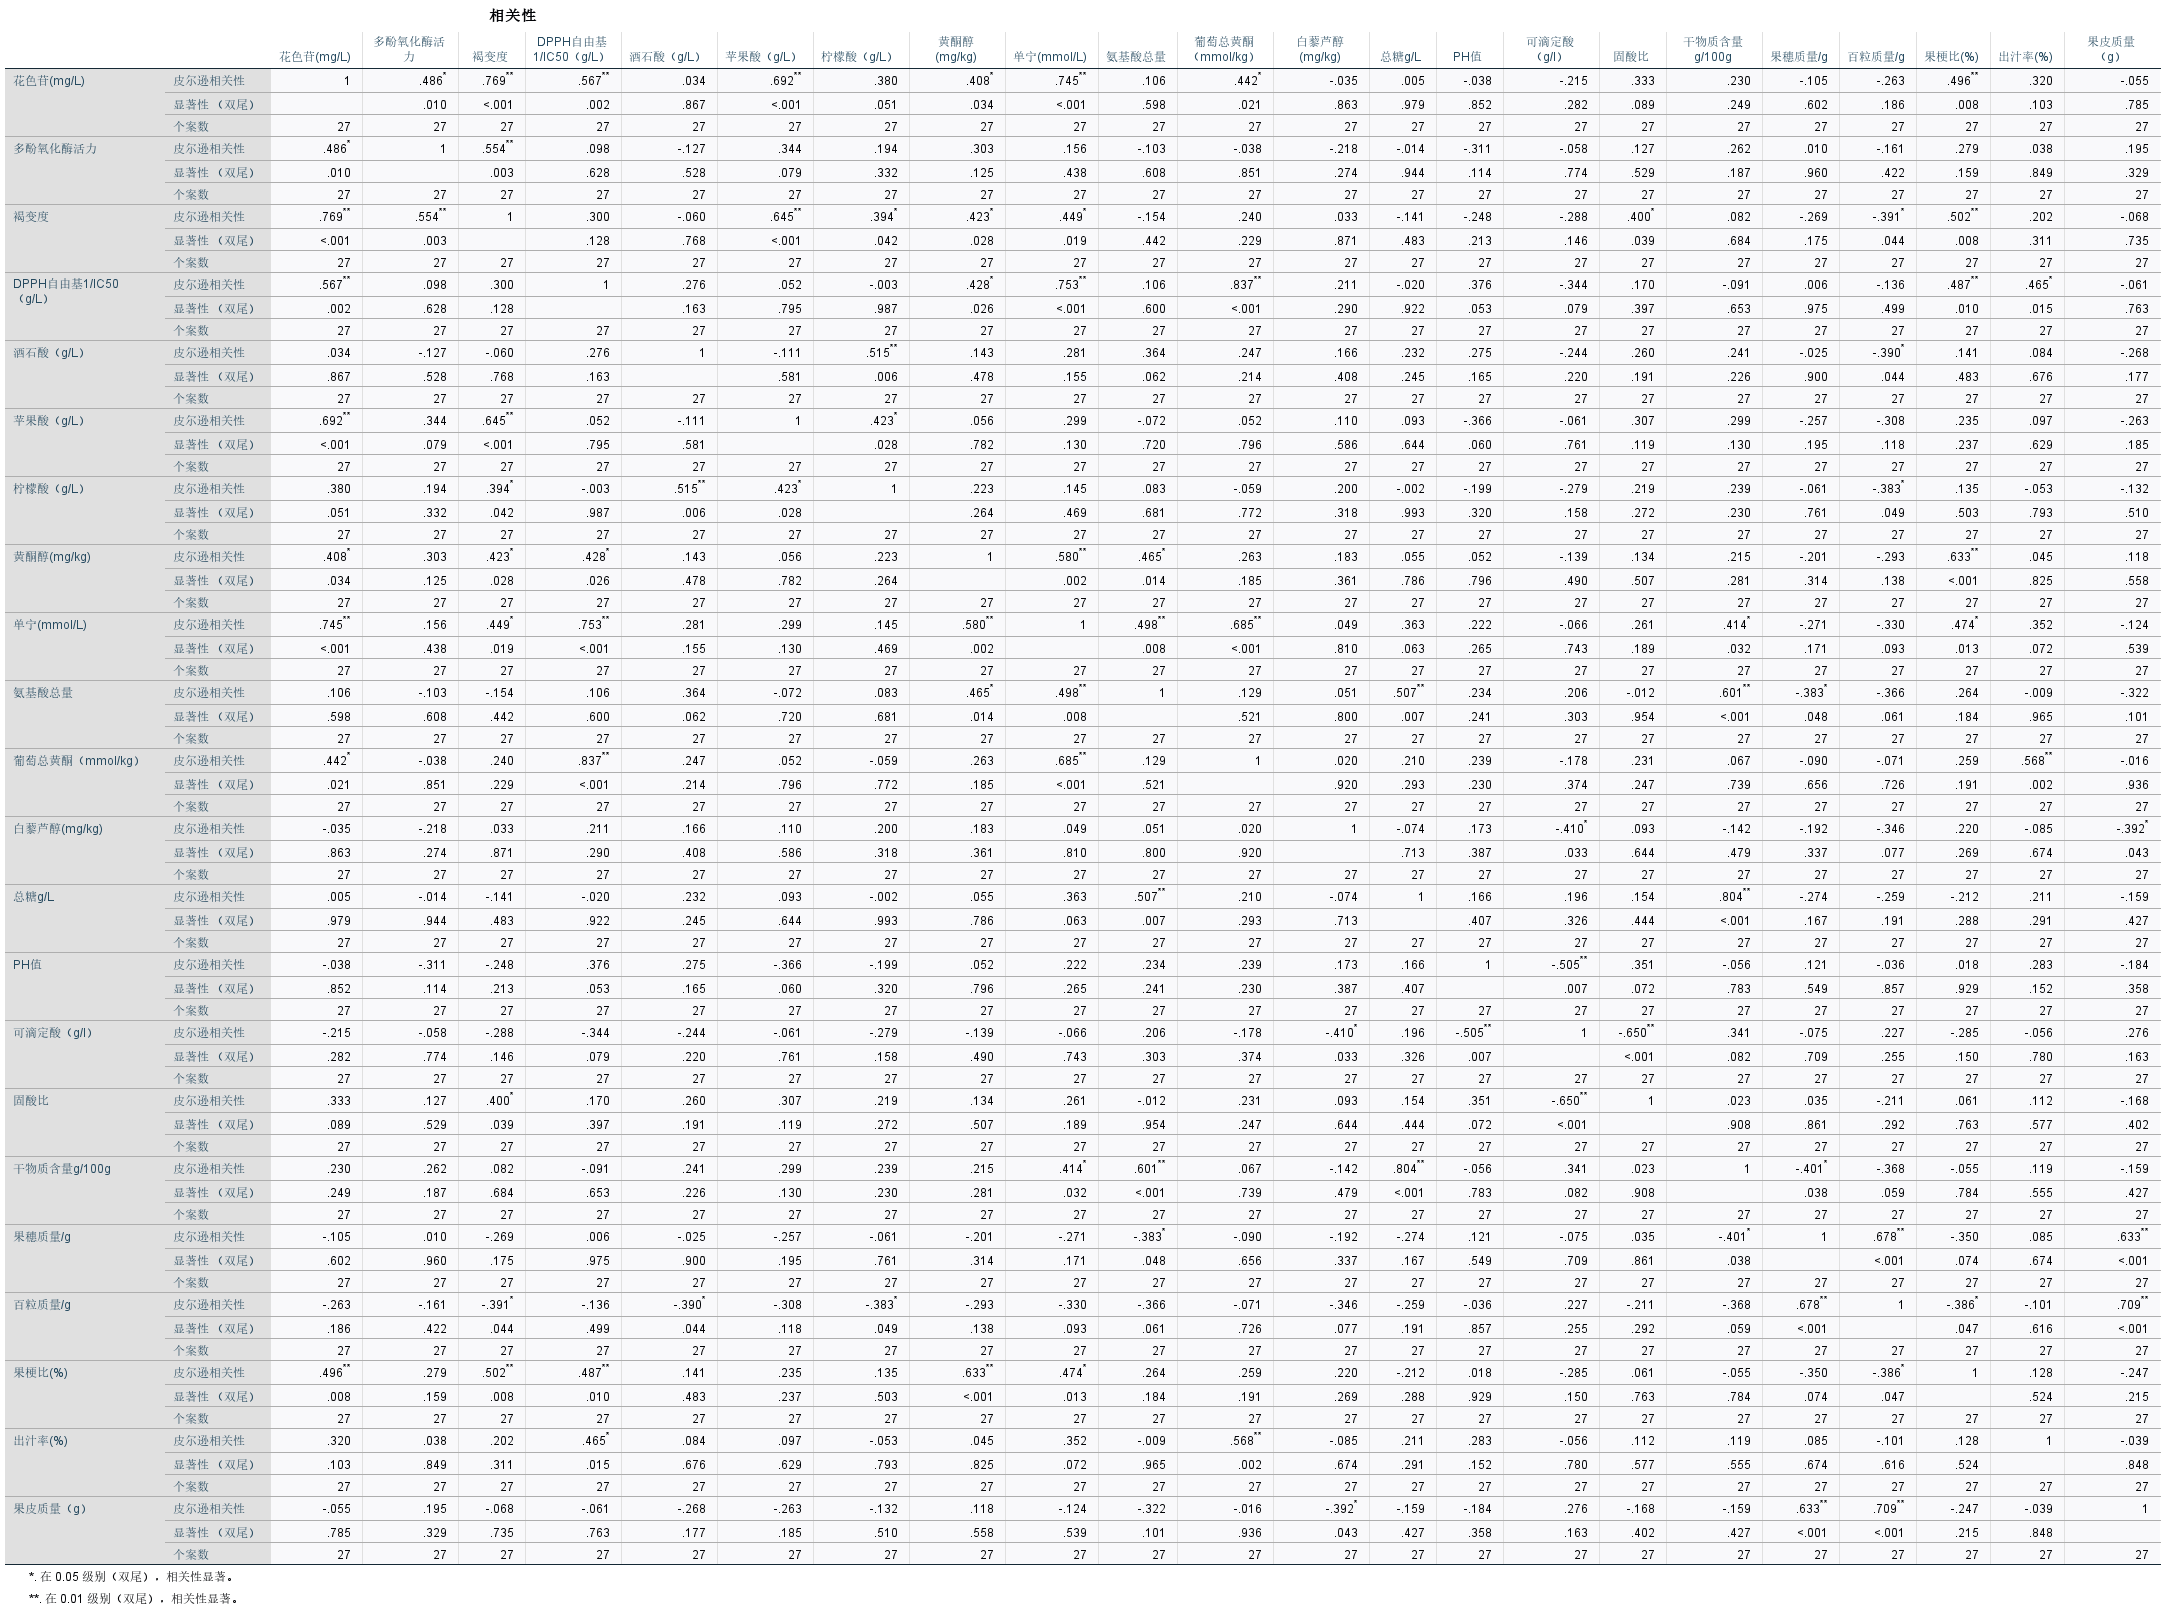
\includegraphics[width=0.9\textwidth]{img/Anthocyanin_correlation_data.png} % 图片相对位置
	\caption{花色苷相关性数据} % 图片标题 
	\label{fig:figure 1} % 图片标签
\end{figure}

\begin{figure}[H]\centering
	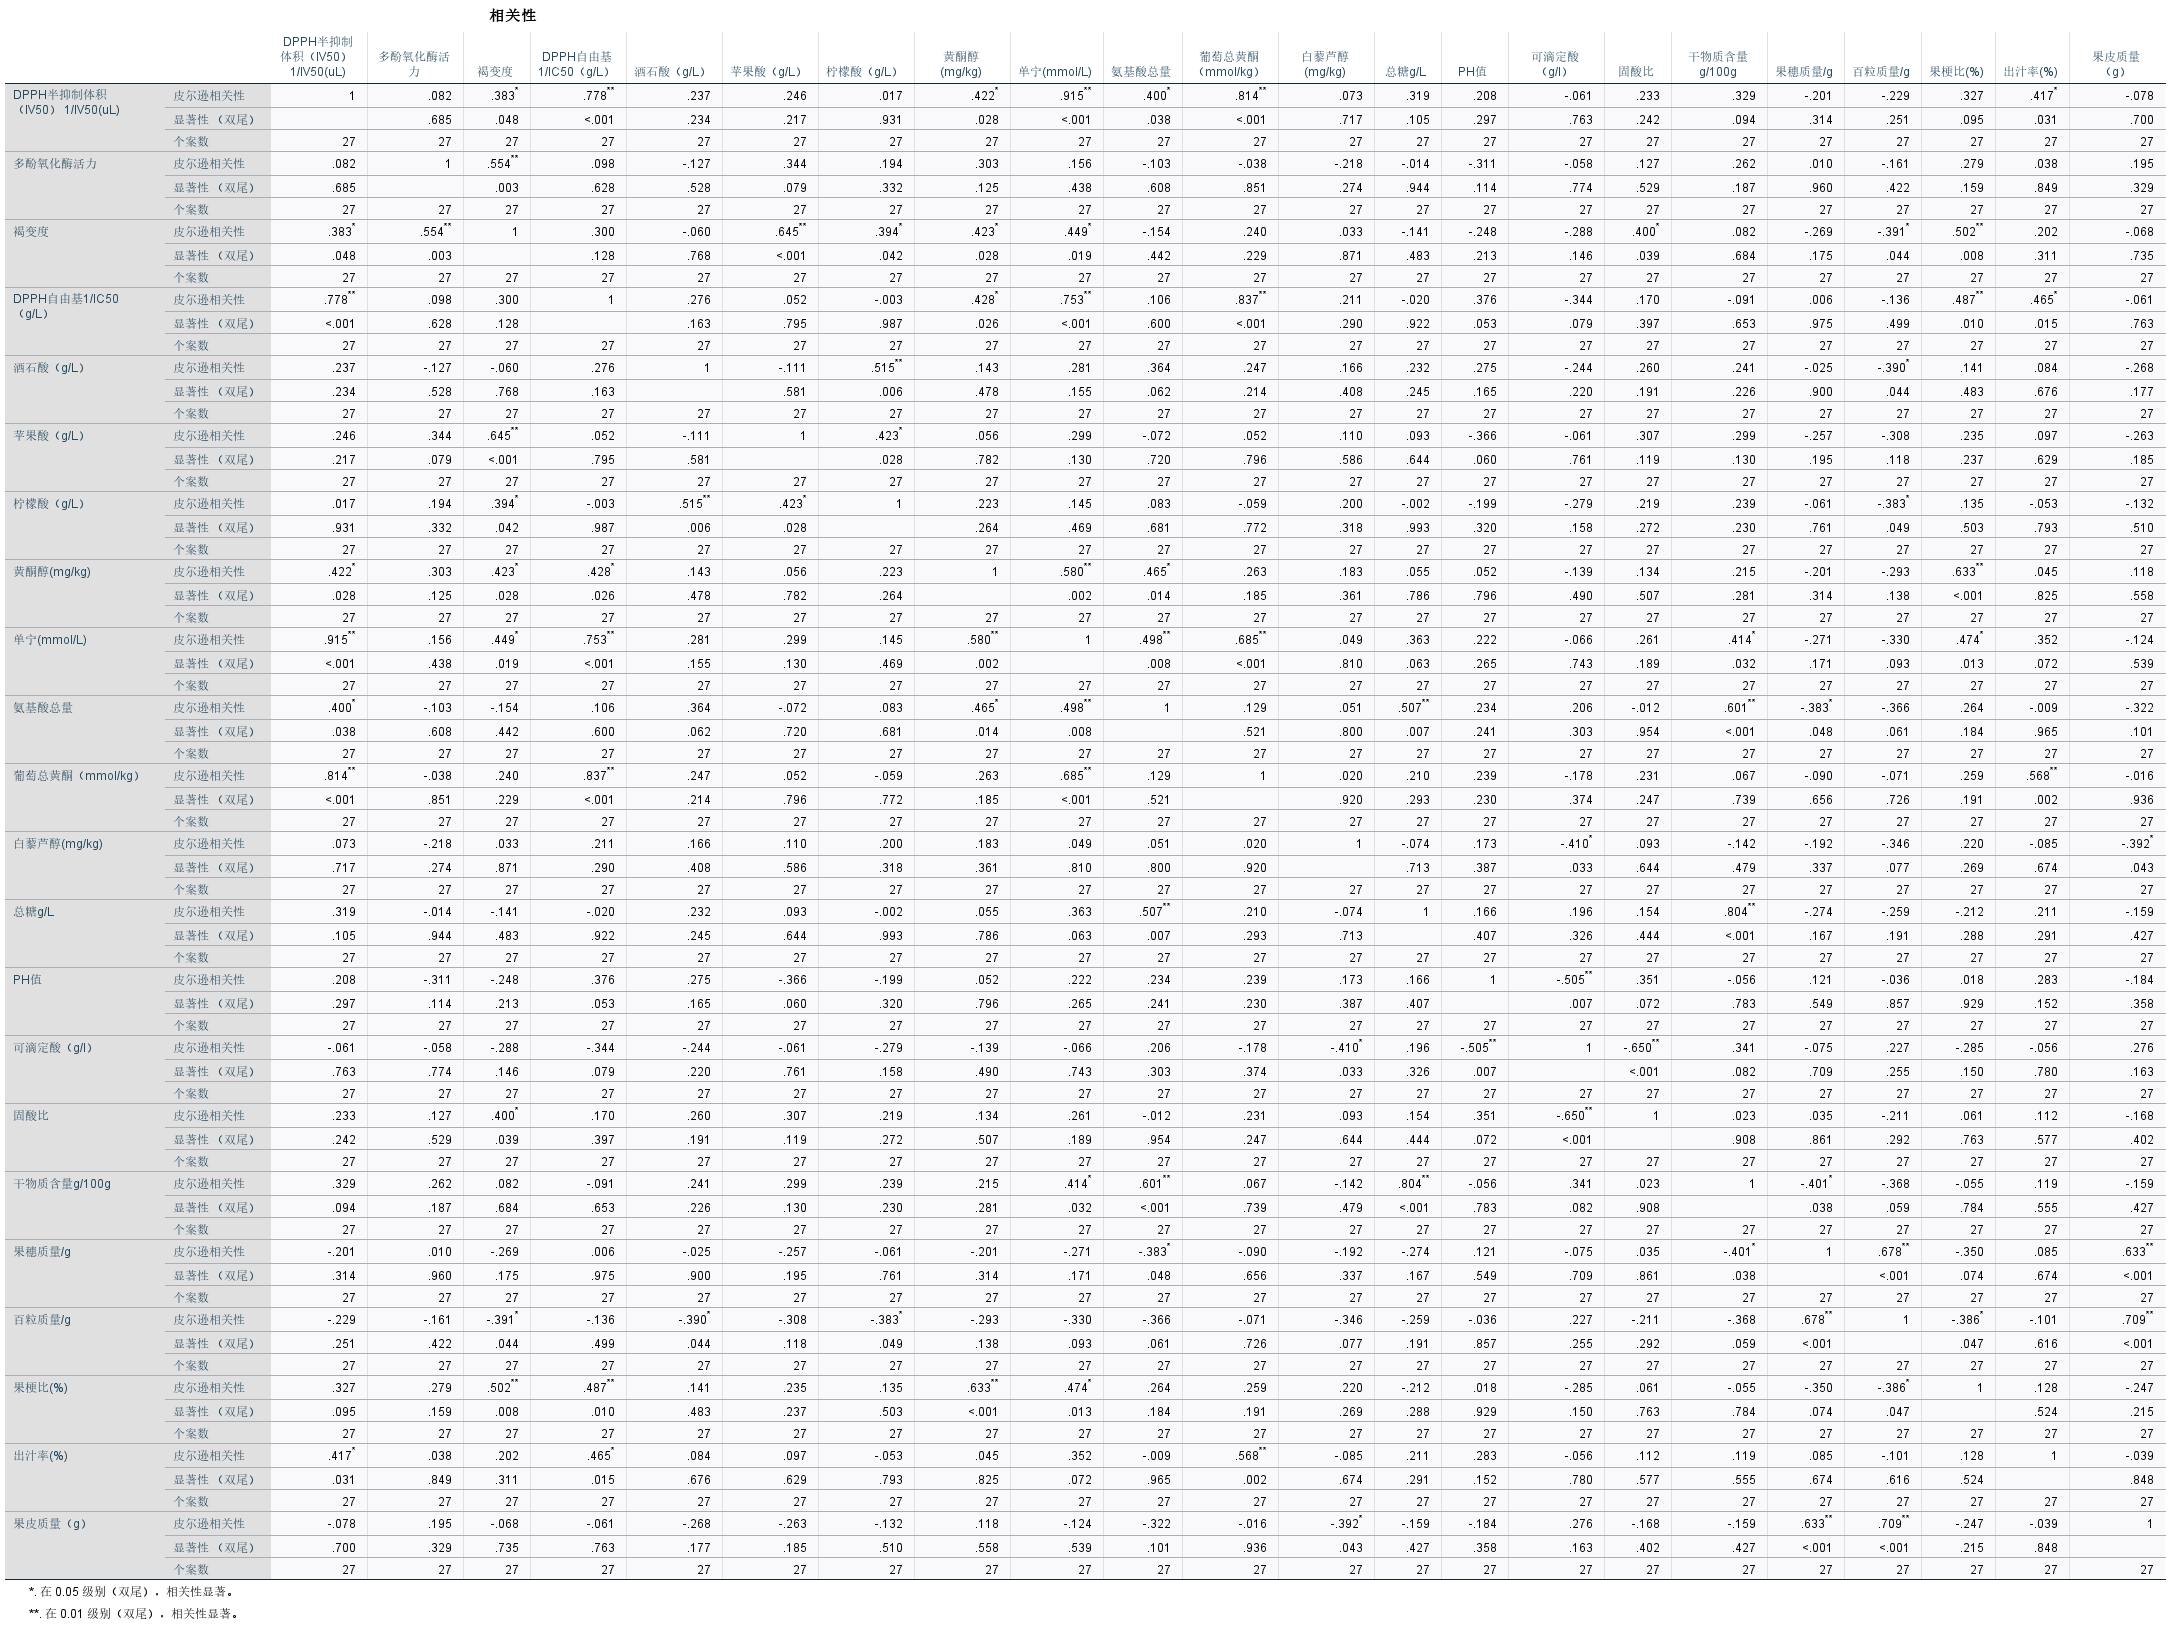
\includegraphics[width=0.9\textwidth]{img/DPPH_semi_inhibitory_volume_correlation_data.png}
	\caption{DPPH半抑制体积相关性数据} % 图片标题 
	\label{fig:figure 2} % 图片标签
\end{figure}


\begin{figure}[H]\centering
	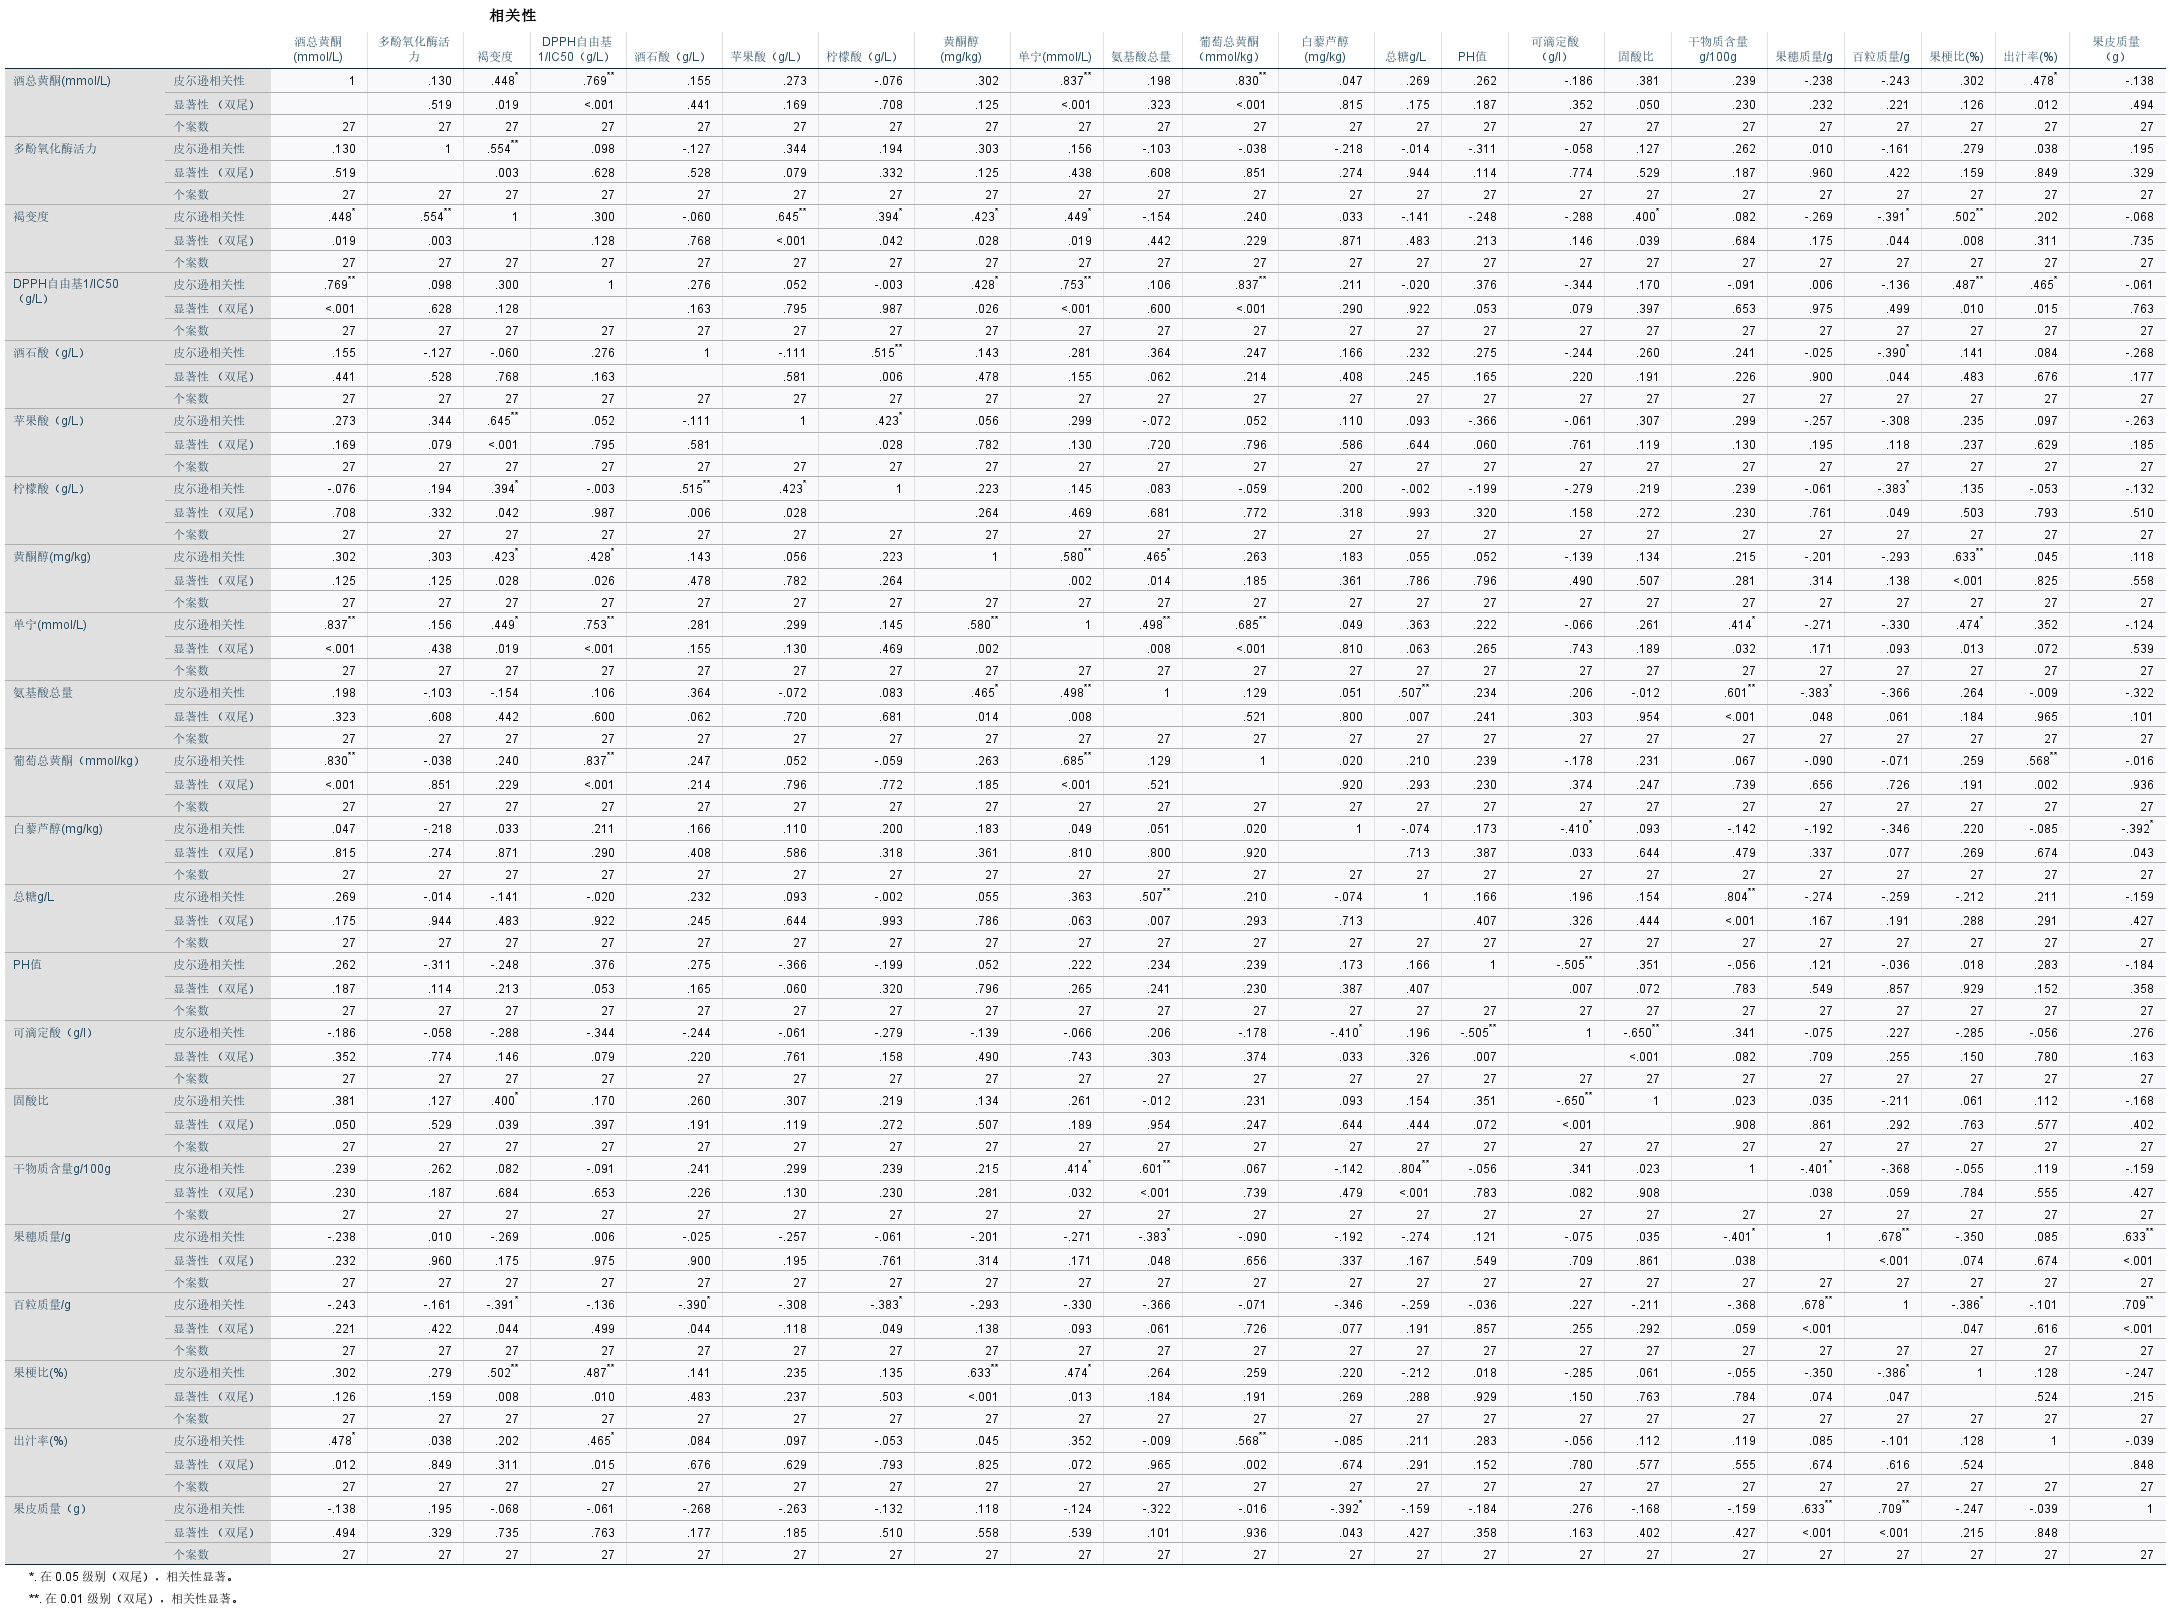
\includegraphics[width=0.9\textwidth]{img/Correlation_data_of_total flavonoids_in_wine.png} % 图片相对位置
	\caption{酒总黄酮相关性数据} % 图片标题 
	\label{fig:figure 3} % 图片标签
\end{figure}

\begin{figure}[H]\centering
	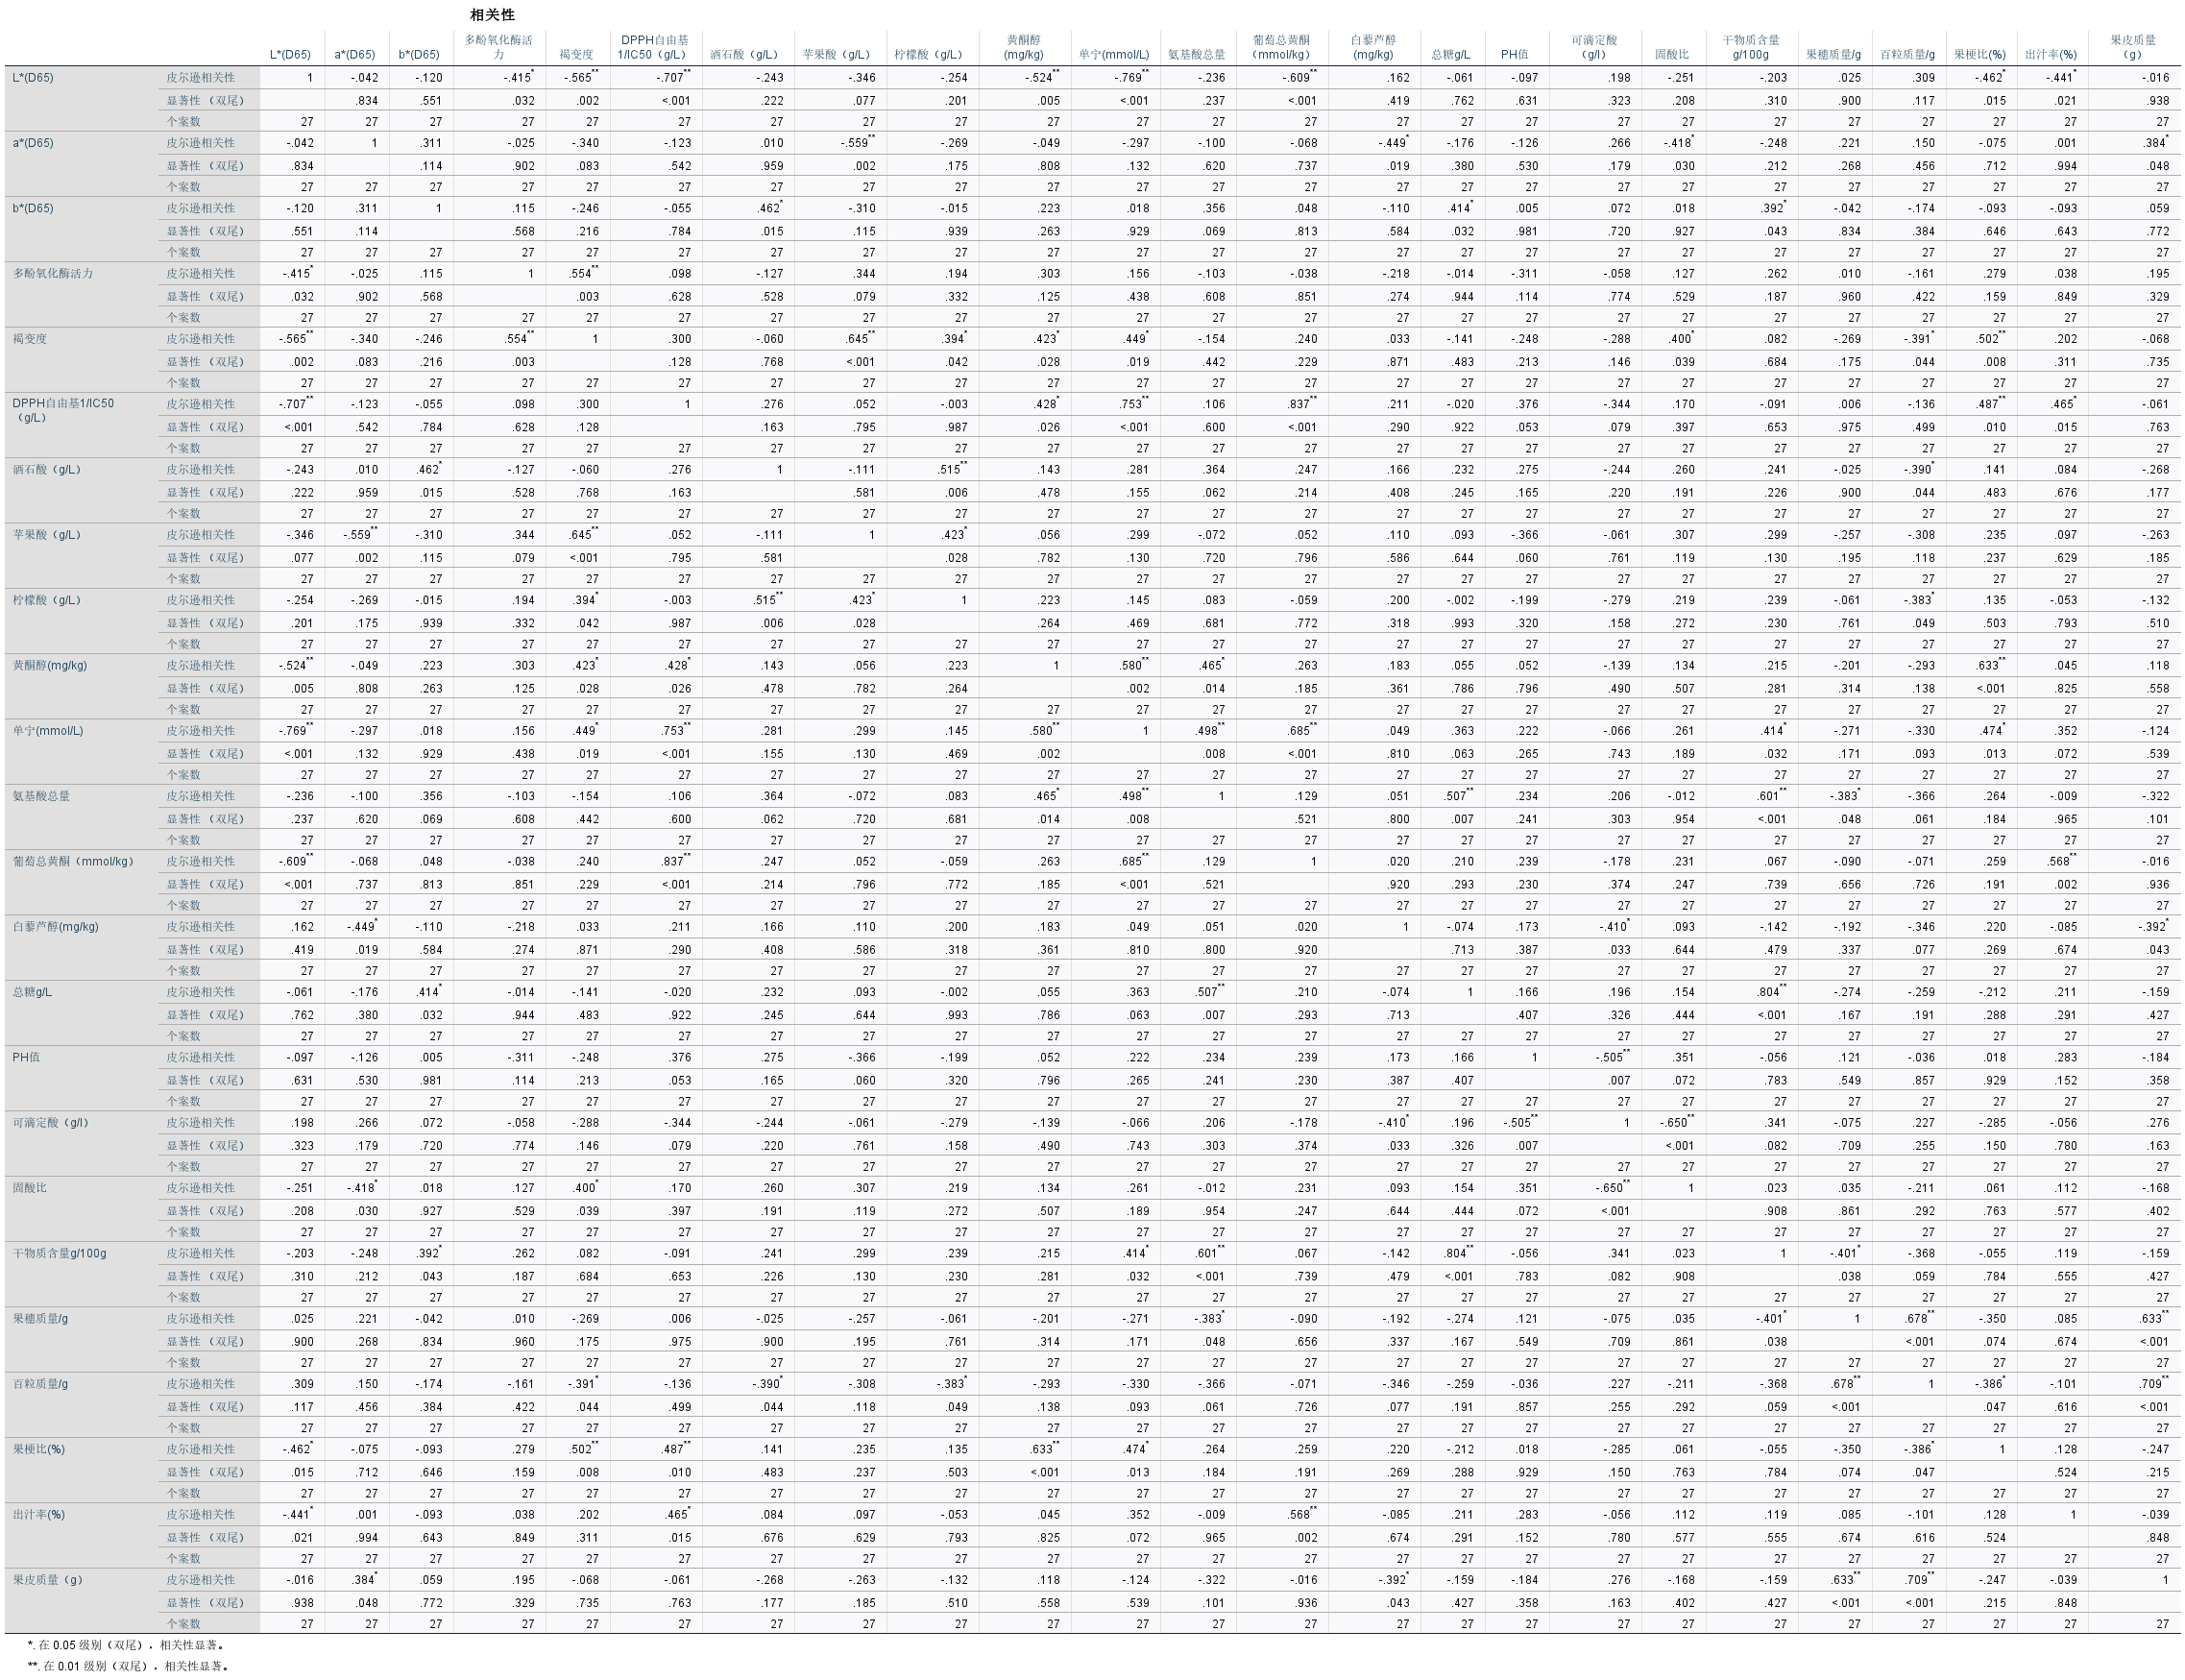
\includegraphics[width=0.9\textwidth]{img/Color_correlation_data.png} % 图片相对位置
	\caption{色泽相关性数据} % 图片标题 
	\label{fig:figure 4} % 图片标签
\end{figure}

\newpage

\subsubsection{结果分析}
对相关性分析的结果进行分析,其重点就是观察其pearson和双侧显著性的值,pearson相关系数的值大,则相关性高,同理观察算观测
双侧显著性则是判断其值的范围,*p<0.05或者**p<0.01都证明其有较好的相关显著性。通过对结果进行分析,得出如下的一些较为明显
的相关性结论:

\begin{itemize}
	\item [1)]{花色苷的指标与褐变度、苹果酸、单宁、果梗比等数据的相关性较为显著}
	\item [2)]{DPPH半抑制体积与多酚氧化酶活力、DPPH自由基、单宁、葡萄总黄酮、白藜芦醇相关性高,与果皮质量和果穗质量等指标都成负相关}
	\item [3)]{酒总黄酮则跟DPPH自由基、单宁、葡萄总黄酮,白藜芦醇等指标相关性高}
	\item [4)]{色泽跟可滴定酸、果穗质量的略微相关,总体数据的相关性不大}
\end{itemize}

按照分析标准来分析,无论是相关性系数和显著程度都选取较为明显的那组数据来进行后面的关系分析。
本小问中,在花色苷则这项数据所给出的相关性指标的相关性都较高,在多元回归中则考虑采取这项数据来进行拟合。

\subsubsection{多元线性回归模型的求解}
在建立模型则需要对模型进行拟合度检验,多元回归方程的显著性检验就是检验样本回归方程的变量的线性关系是否显著,
需要根据样本来判断方程中的多个回归系数中至少有一个不等于0,主要是说明样本回归方程的显著性。
检验的方法用方差分析,这时因变量的总体为回归平方和与误差平方和,即表示为:
\begin{equation}
	L_xx = Q+U
\end{equation}
其中该公式又可以表示为:
\begin{equation}
	L_xx=\sum_{i=1}^{N}(y_i-\bar{y})^2
\end{equation}
\begin{equation}
	Q=\sum_{i=1}^{N}(y_i-\hat{y})^2
\end{equation}
\begin{equation}
	U=\sum_{i=1}^{N}(\hat{y_i}-\bar{y})^2
\end{equation}

对花色苷和其相关性较高的指标进行拟合,依据德宾沃森残差,离群值为3标准差进行模型拟合,来根据其R方及其
德宾沃森残差来观察其拟合的契合度。
另外进行单因素方差分析(ANOVA)来观测F检验对整个回归进行显著性检验,考虑的k个变量自变量是否有显著性线性关系
F检测通过与F边界值来进行比对判断其水平显著性
\[\left\{\begin{array}{llcl}
		F_0.05(k,n-k-1) \le F \le F_0.01(k,n-k-1){认为回归在0.05水平上显著} \\

		F_0.1(k,n-k-1) \le F \le F_0.05(k,n-k-1){认为回归在0.01水平上显著}  \\

		F<F_0.1(k,n-k-1){则回归不显著}                                      \\
	\end{array} \right.\]
\subsubsection{单因素方差分析}
对花色苷等多项相关性数据进行ANOVA分析,观察F检测值和显著性,通过三组不同数据的模型,对数据进行共线性诊断,依据
VIF值来确定较为合理的自变量,来进行试验观察。
得出如下的结果:
\begin{figure}[H]\centering

	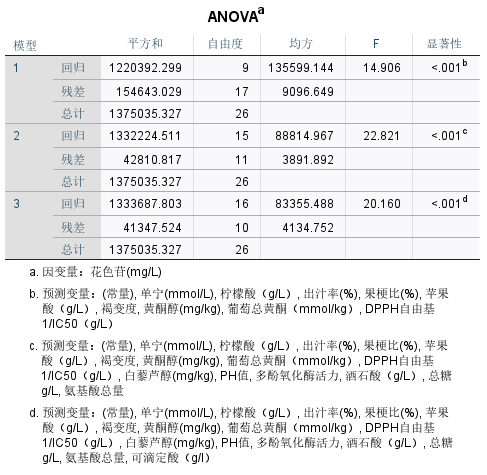
\includegraphics[width=0.52\textwidth,height=0.45\textwidth]{img/ANOVA.png} % 图片相对位置

	\caption{ANOVA} % 图片标题 	
	\label{fig:figure 5} % 图片标签
\end{figure}

分析观察三组回归的数据,发现三个模型的显著性都是<0.01,其F检测值分别为:14.906、22.821、20.160。根据该结果和显著性p值可以
拒绝原假设,认为被解释变量个解释变量间存在显著的线性关系,可建立线性回归模型。

如下为残差统计图:
\begin{figure}[H]\centering
	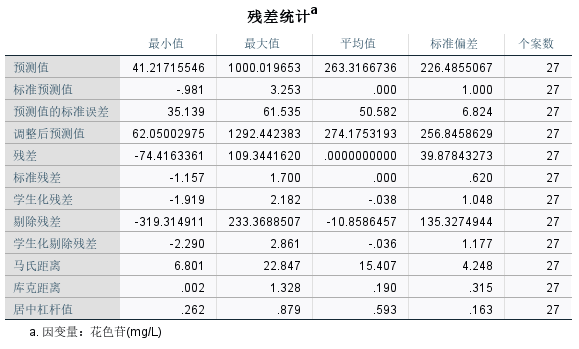
\includegraphics[width=0.52\textwidth,height=0.45\textwidth]{img/Residuals_Statistics.png} % 图片相对位置
	\caption{残差统计} % 图片标题 	
	\label{fig:figure 6} % 图片标签
\end{figure}
在经过处理后的数据是比较合理的。

\subsubsection{多元回归拟合}
花色苷作为因变量,褐变度、苹果酸、单宁、果梗比、DPPH自由基、葡萄总黄酮、多酚氧化酶活力、总酚等相关性较为显著等数据作为自变量来进行多元回归拟合。
在进行比对后发现并无需要严格剔除的数据,则进行多元线性回归变量筛选结果及系数的拟合求解。
观察系数表和其显著性指标,通过${R^2}$来判断其回归拟合的契合度,往往${R^2}$越贴近于1,契合度越高。
确定酿酒葡萄与葡萄酒理化指标的联系则将系数组合成回归方程即可。


\begin{figure}[H]\centering
	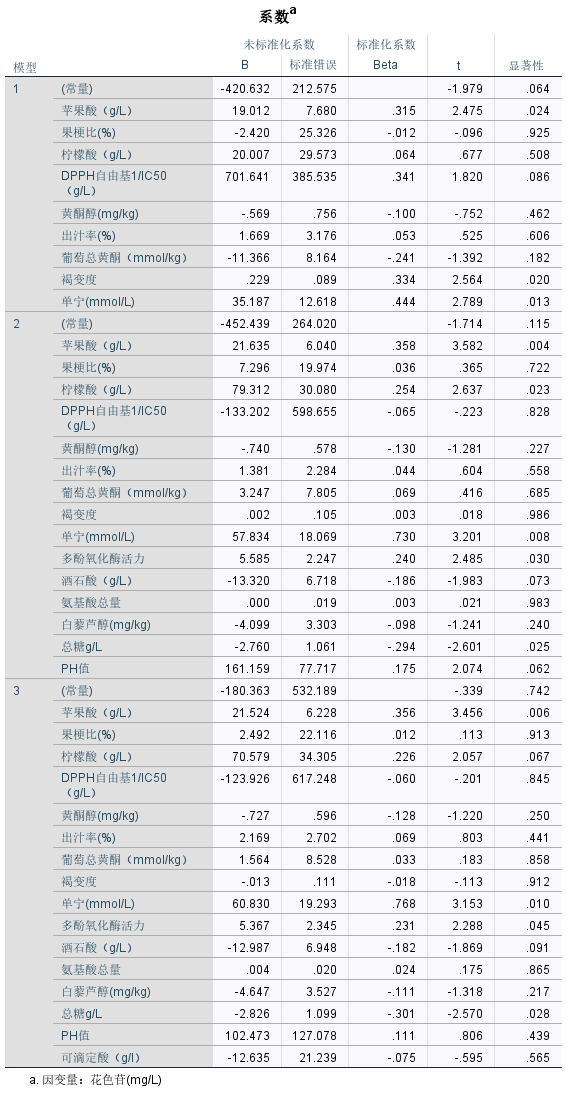
\includegraphics[width=0.8\textwidth,height=1.07\textwidth]{img/Coefficient_table.png} % 图片相对位置
	\caption{系数} % 图片标题 	
	\label{fig:figure 8} % 图片标签
\end{figure}

通过如下图表判断${R^2}$
\begin{figure}[H]\centering
	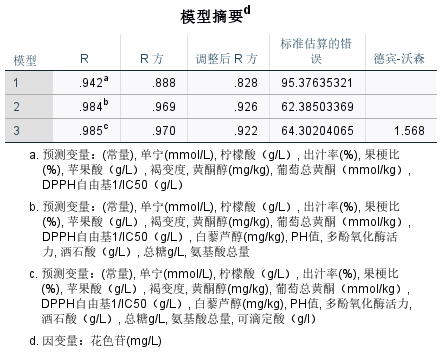
\includegraphics[width=0.52\textwidth,height=0.45\textwidth]{img/abstrat.png} % 图片相对位置
	\caption{模型摘要} % 图片标题 	
	\label{fig:figure 7} % 图片标签
\end{figure}
通过上述分析得出,三组数据的${R^2}$都相对趋近于1,具有较高的契合度。比对之后选择模型3的数据来进行方程的建立。
由如下的系数表来得到系数关系。
选取苹果酸、果梗比、柠檬酸、DPPH自由基、黄酮醇、出汁率.......等指标作为自变量${x_1,x_2,,,,,x_n}$构建如下方程:

\begin{equation}
	y=21.524{x_1}+2.49{x_2}+70.579{x_3}-123.926{x_4}-7.27{x_5}+2.169{x_6}+1.564{x_7}-0.013{x_8}+60.83{x_9}
\end{equation}
\begin{equation}
	+5.367{x_{10}}-12.987{x_{11}}+0.004{x_{12}}-4.647{x_{13}}-2.826{x_{14}}+102.473{x_{15}}-12.635{x_{16}}-420.632
\end{equation}

其中$y$为因变量花色苷,${x_1,x_2,,,,,x_n}$则为自变量苹果酸、果梗比、柠檬酸、DPPH自由基、黄酮醇、出汁率.......
通过该方程可以反映出葡萄酒的某些指标与酿酒葡萄理化指标之间的关系。



% \end{thebibliography}
\subsection{问题四的求解}
针对该小问,要分析酿酒葡萄和葡萄酒的理化指标对葡萄酒质量的影响,并判断能否将其用来作为评价葡萄酒的质量的标准。
采用问题二所提出的主成分分析法,对酿酒葡萄和葡萄酒理化指标进行主成分提取,通过对主成分中的占比分析来判断对质量
影响较大的理化指标。后通过回归分析法,对葡萄酒重新进行打分,比对给出的数据来判断其以理化指标来评价质量是否合理。
\subsubsection{主成分分析}
首先进行KMO和Bartlett的检验,对于KMO值:0.8上则合适做主成分分析,0.7-0.8之间一般适合
0.6-0.7之间不太适合,0.5-0.6之间表示差,0.5下表示极不适合,对于 Bartlett的检验(p < 0.05,严格来说p < 0.01),
若显著性小于0.05或0.01,拒绝原假设,则说明可以做主成分分析,若不拒绝原假设,则说明这些变量可能独立提供一些信息,
不适合做主成分分析。后通过分析方差解释表格和碎石图,确定主成分的数量方差解释表格主要是看主成分对于变量解释的贡献率。
通过下图判断得出主成分分析条件合理。

\begin{table*}[h!]
	\begin{center}
		\caption{KMO检验和Bartlett的检验}
		\begin{tabular}{c c c}
			\hline
			KMO值                                                    & 0.851             \\
			\hline
			\multicolumn{1}{c|}{\multirow{3}{*}{Bartlett球形度检验}} & 近似卡方 & 1.238  \\
			\multicolumn{1}{c|}{}                                    & df       & 165.54 \\
			\multicolumn{1}{c|}{}                                    & p        & 0.02   \\
			\hline
		\end{tabular}
	\end{center}
\end{table*}
KMO检验的结果显示,KMO的值为0.851,同时,Bartlett球形检验的结果显示,显著性P值为0.02,水平上呈现显著性,不接受原假设,也就是变量间耦合程度搞,则可以从中提取公因子,主成分分析有效.

据此进行主成分分析得到结果如下, 下表为总方差解释表格,主要是看主成分对于变量解释的贡献率(可以理解为究竟需要多少主成分才能把变量表达为100\%),一般都要表达到80\%以上才可以,否则就要调整因子数据。 一般情况下,方差解释率越高,说明该主成分越重要,权重占比也应该越高。

方差解释表中,在主成分9时,总方差解释的特征根低于1.0,变量解释的贡献率达到86.558\%,仅为参考,若特征根小于1.0临界值过大,也可以集合具体情况具体分析。

\begin{table}[!ht]
	\centering
	\caption{方差解释}
	% \resizebox{\textwidth}{35mm}{
	% 	\resizebox{\textheight}{70mm}{
	\begin{tabular}{|r|r|r|r|}
		\hline
		成分   & 特征根     & ~        & ~        \\ \hline
		特征根 & 方差百分比 & 累积     & ~        \\ \hline
		1      & 6.812      & 21.973\% & 21.973\% \\ \hline
		2      & 5.785      & 18.662\% & 40.635\% \\ \hline
		3      & 3.872      & 12.491\% & 53.126\% \\ \hline
		4      & 2.535      & 8.176\%  & 61.302\% \\ \hline
		5      & 2.199      & 7.092\%  & 68.395\% \\ \hline
		6      & 1.722      & 5.556\%  & 73.951\% \\ \hline
		7      & 1.703      & 5.494\%  & 79.445\% \\ \hline
		8      & 1.214      & 3.916\%  & 83.36\%  \\ \hline
		9      & 0.991      & 3.198\%  & 86.558\% \\ \hline
		10     & 0.887      & 2.862\%  & 89.419\% \\ \hline
		11     & 0.601      & 1.939\%  & 91.358\% \\ \hline
		12     & 0.543      & 1.753\%  & 93.111\% \\ \hline
		13     & 0.480      & 1.548\%  & 94.659\% \\ \hline
		14     & 0.376      & 1.213\%  & 95.872\% \\ \hline
		15     & 0.328      & 1.059\%  & 96.93\%  \\ \hline
		16     & 0.208      & 0.672\%  & 97.602\% \\ \hline
		17     & 0.170      & 0.549\%  & 98.151\% \\ \hline
		18     & 0.162      & 0.522\%  & 98.673\% \\ \hline
		19     & 0.129      & 0.417\%  & 99.091\% \\ \hline
		20     & 0.093      & 0.299\%  & 99.39\%  \\ \hline
		21     & 0.078      & 0.252\%  & 99.642\% \\ \hline
		22     & 0.054      & 0.174\%  & 99.816\% \\ \hline
		23     & 0.027      & 0.086\%  & 99.901\% \\ \hline
		24     & 0.014      & 0.046\%  & 99.947\% \\ \hline
		25     & 0.010      & 0.033\%  & 99.98\%  \\ \hline
		26     & 0.006      & 0.02\%   & 100.0\%  \\ \hline
		27     & 0.000      & 0.0\%    & 100.0\%  \\ \hline
		28     & -0.000     & -0.0\%   & 100.0\%  \\ \hline
		29     & -0.000     & -0.0\%   & 100.0\%  \\ \hline
		30     & -0.000     & -0.0\%   & 100.0\%  \\ \hline
		31     & -0.000     & -0.0\%   & 100.0\%  \\ \hline
	\end{tabular}
\end{table}

\begin{equation}
	\begin{aligned}
		A_n & =\pi_{\mbox{第一年}} - \pi_{\mbox{最后一年}}       \\
		R_n & =\frac{\pi_{\mbox{第一年}}}{\pi_{\mbox{最后一年}}}
	\end{aligned}
\end{equation}


下面碎石图是根据各主成分对数据变异的解释程度绘制的图。其作用是根据特征值下降的坡度来确认需要选择的主成分个数,我们结合方差解释表用于确认或调整主成分个数。 每一个主成分为一个点,通过“坡度趋于平缓”的未知判断提取主成分的数量。我们综合方差解释以及碎石图,最终确定使用前8个特征作为表征值。

\begin{figure}[H]\centering

	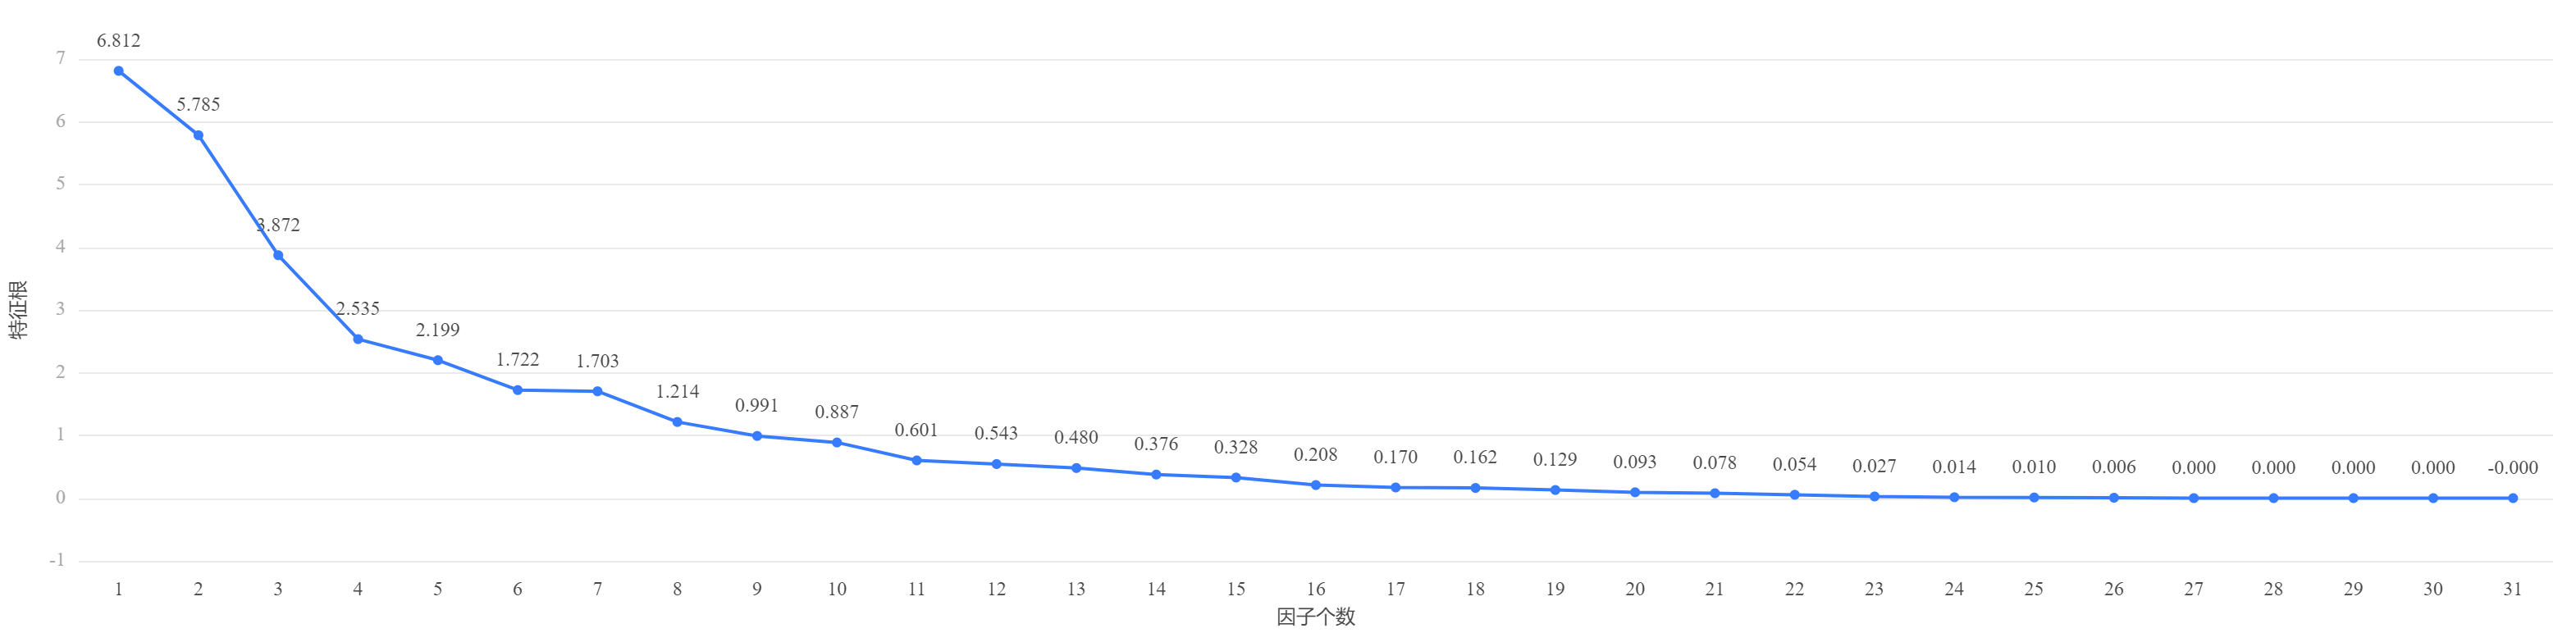
\includegraphics[width=0.52\textwidth,height=0.45\textwidth]{img/4/solid.png} % 图片相对位置
	\caption{碎石图} % 图片标题 	
	\label{fig:figure 5} % 图片标签
\end{figure}

下表为因子载荷系数表,可以分析到每个主成分中隐变量的重要性。假设前文确定得到n个因子,因子 i 中a、b、c、d的因子载荷系数较大,因此可将主成分 i 进行总结重命名。


\begin{table}[!ht]
	\centering
	\caption{因子权重分析}
	\resizebox{\textwidth}{65mm}{
		\resizebox{\textheight}{150mm}{
			\begin{tabular}{|c|c|c|c|c|c|c|c|c|c|}
				\hline
				~              & 主成分1 & 主成分2 & 主成分3 & 主成分4 & 主成分5 & 主成分6 & 主成分7 & 主成分8 & 共同度(公因子方差) \\ \hline
				胱氨酸         & 0.382   & -0.203  & -0.141  & 0.391   & -0.18   & -0.154  & 0.307   & 0.387   & 0.66                 \\ \hline
				缬氨酸         & 0.814   & -0.333  & 0.058   & -0.152  & 0.021   & -0.166  & -0.077  & 0.201   & 0.874                \\ \hline
				丙氨酸         & 0.587   & -0.048  & -0.459  & 0.055   & -0.189  & 0.13    & -0.189  & -0.229  & 0.702                \\ \hline
				天门冬氨酸     & 0.602   & 0.261   & -0.157  & 0.169   & -0.582  & 0.074   & 0.065   & -0.097  & 0.842                \\ \hline
				氨基酸总量     & 0.199   & 0.097   & 0.303   & 0.844   & -0.029  & -0.147  & -0.205  & -0.055  & 0.921                \\ \hline
				丝氨酸         & 0.703   & -0.321  & -0.144  & 0.356   & -0.087  & -0.094  & -0.055  & -0.018  & 0.765                \\ \hline
				蛋氨酸         & 0.756   & 0.181   & 0.047   & -0.094  & 0.339   & 0.021   & -0.185  & -0.076  & 0.771                \\ \hline
				苏氨酸         & 0.426   & 0.492   & -0.523  & 0.2     & 0.311   & -0.091  & -0.21   & -0.168  & 0.914                \\ \hline
				白藜芦醇       & 0.127   & 0.054   & -0.021  & 0.136   & -0.24   & 0.71    & 0.14    & 0.481   & 0.85                 \\ \hline
				亮氨酸         & 0.789   & -0.338  & 0.054   & -0.23   & 0.044   & -0.208  & -0.051  & 0.119   & 0.854                \\ \hline
				谷氨酸         & 0.658   & 0.109   & -0.651  & -0.011  & 0.006   & 0.118   & -0.054  & -0.074  & 0.891                \\ \hline
				多酚氧化酶活力 & -0.31   & 0.477   & -0.202  & -0.144  & 0.476   & -0.307  & -0.115  & 0.239   & 0.776                \\ \hline
				葡萄总黄酮     & 0.378   & 0.588   & 0.529   & -0.189  & -0.275  & -0.13   & 0.005   & 0.008   & 0.897                \\ \hline
				苯丙氨酸       & 0.259   & 0.105   & 0.127   & -0.061  & -0.237  & 0.05    & 0.647   & -0.598  & 0.933                \\ \hline
				单宁           & 0.303   & 0.744   & 0.188   & 0.031   & -0.137  & -0.032  & -0.167  & -0.139  & 0.748                \\ \hline
				蛋白质         & 0.033   & 0.439   & 0.687   & -0.202  & 0.211   & 0.347   & -0.019  & -0.032  & 0.873                \\ \hline
				DPPH自由基     & 0.293   & 0.665   & 0.538   & -0.209  & -0.134  & 0.118   & -0.118  & 0.194   & 0.944                \\ \hline
				褐变度         & -0.018  & 0.75    & -0.293  & -0.176  & 0.233   & 0.077   & -0.02   & -0.001  & 0.74                 \\ \hline
				总酚           & 0.421   & 0.71    & 0.441   & -0.074  & -0.169  & -0.168  & -0.104  & 0.043   & 0.95                 \\ \hline
				甘氨酸         & 0.528   & 0.342   & -0.521  & 0.03    & -0.169  & 0.12    & 0.104   & 0.33    & 0.831                \\ \hline
				脯氨酸         & 0.008   & 0.121   & 0.375   & 0.837   & -0.05   & -0.168  & -0.184  & -0.049  & 0.922                \\ \hline
				VC含量         & -0.104  & -0.07   & -0.087  & -0.112  & -0.355  & 0.567   & -0.437  & -0.124  & 0.689                \\ \hline
				异亮氨酸       & 0.688   & -0.278  & -0.05   & -0.279  & 0.065   & -0.251  & 0.115   & 0.117   & 0.725                \\ \hline
				酪氨酸         & 0.369   & 0.038   & 0.226   & -0.354  & -0.316  & -0.27   & 0.408   & 0.015   & 0.654                \\ \hline
				花色苷         & 0.172   & 0.925   & -0.041  & -0.027  & 0.117   & -0.031  & -0.107  & -0.003  & 0.915                \\ \hline
				酒石酸         & 0.263   & 0.068   & 0.556   & 0.343   & 0.383   & 0.176   & 0.367   & 0.154   & 0.837                \\ \hline
				柠檬酸         & 0.15    & 0.305   & -0.101  & 0.272   & 0.556   & 0.304   & 0.527   & -0.097  & 0.889                \\ \hline
				赖氨酸         & 0.659   & -0.401  & 0.312   & 0.114   & 0.254   & 0.227   & -0.082  & -0.1    & 0.838                \\ \hline
				组氨酸         & 0.714   & -0.472  & 0.226   & -0.176  & 0.333   & 0.047   & -0.13   & -0.103  & 0.955                \\ \hline
				苹果酸         & 0.15    & 0.62    & -0.645  & 0.066   & 0.11    & 0.04    & 0.229   & -0.006  & 0.894                \\ \hline
				精氨酸         & 0.537   & -0.52   & 0.156   & -0.166  & 0.268   & 0.294   & -0.123  & -0.067  & 0.788                \\ \hline
			\end{tabular}}}
\end{table}


下图为载荷矩阵热力图,可以分析到每个主成分中隐变量的重要性。我们结合热力图进行各因子的隐变量分析。

\begin{figure}[H]\centering

	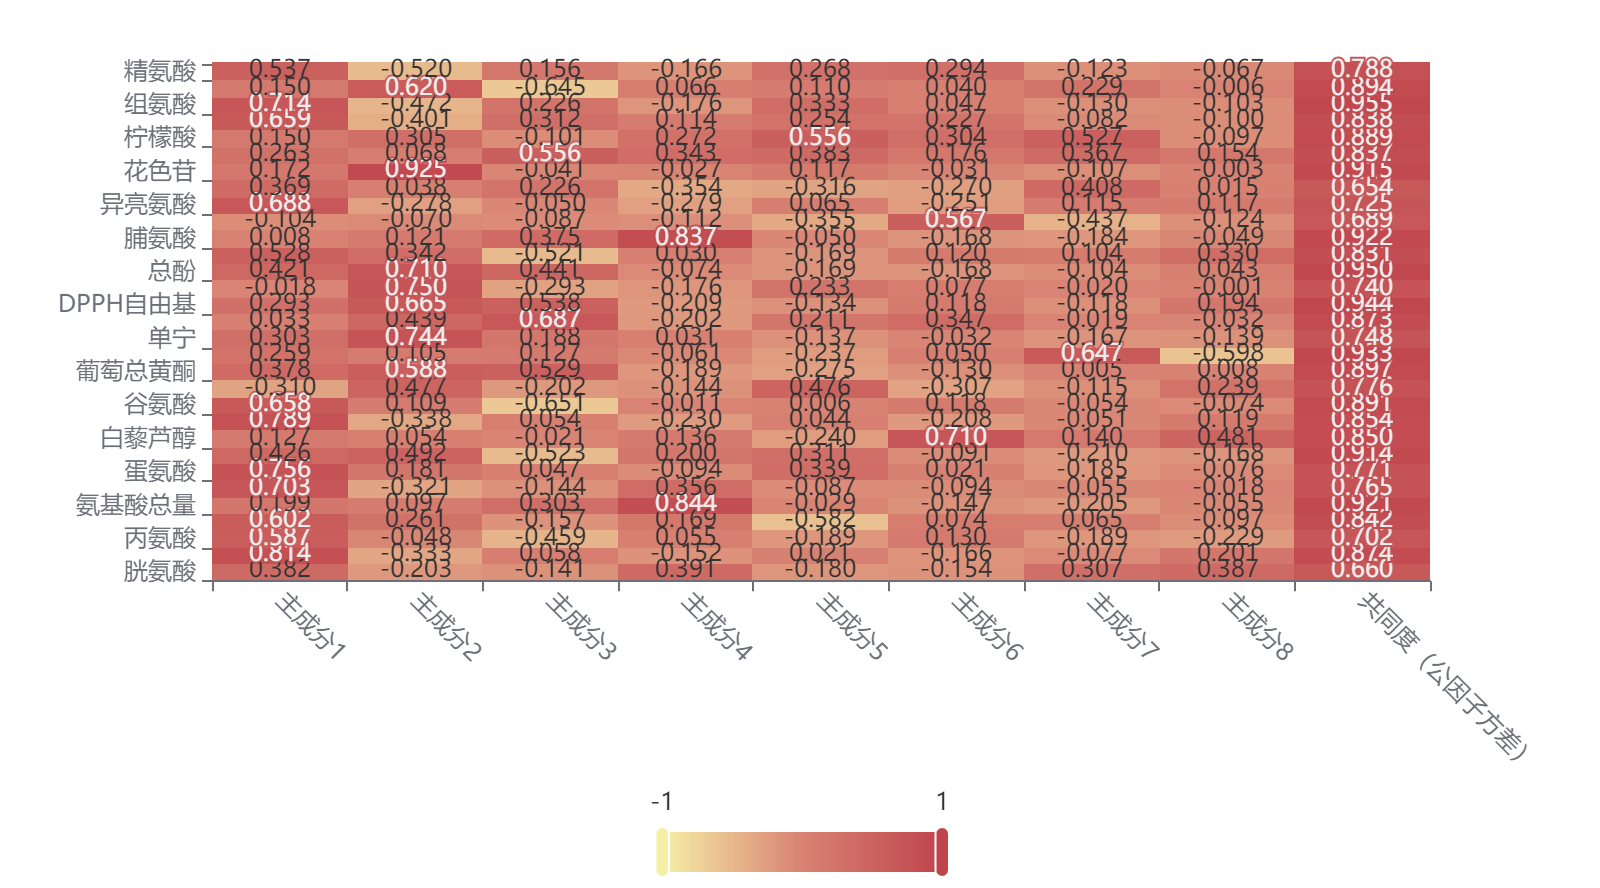
\includegraphics[width=0.52\textwidth,height=0.52\textwidth]{img/4/heatmaps.png} % 图片相对位置

	\caption{热力图} % 图片标题 	
	\label{fig:figure 5} % 图片标签
\end{figure}

因子载荷图通过将多因子降维成双主成分或者三主成分,通过象限图的方式呈现主成分的空间分布。

\begin{figure}[H]\centering

	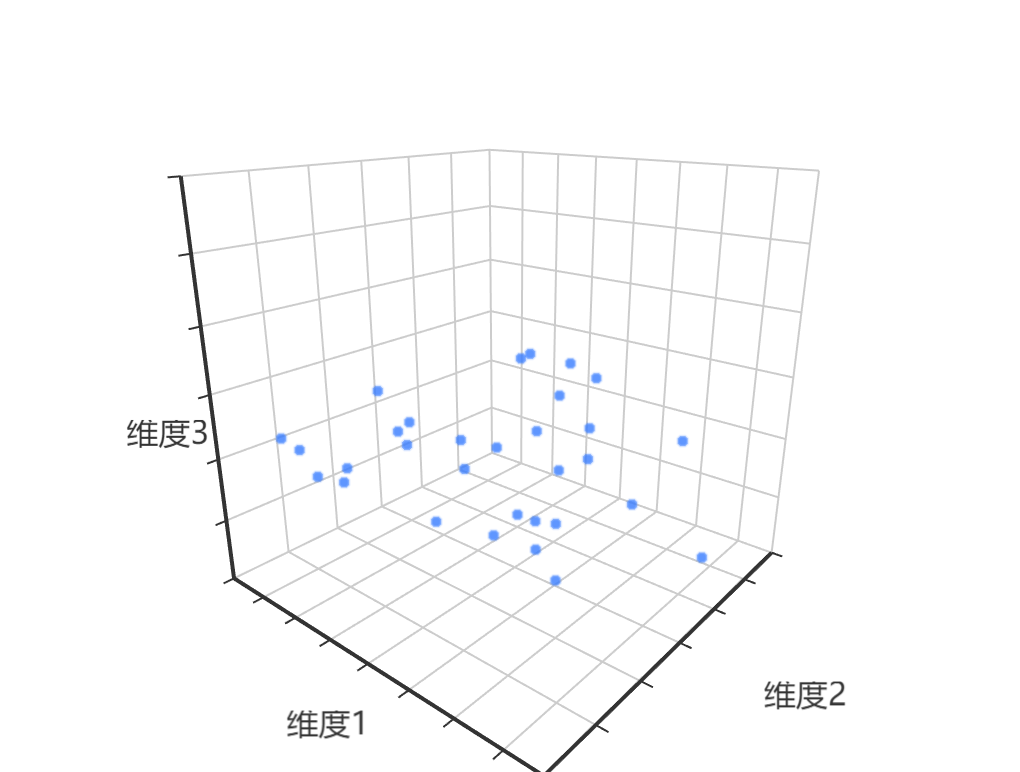
\includegraphics[width=0.52\textwidth,height=0.45\textwidth]{img/4/3d_analysise.png} % 图片相对位置

	\caption{因子载荷象限分析} % 图片标题 	
	\label{fig:figure 5} % 图片标签
\end{figure}


下表为成分矩阵表,意在说明各个成分的所包含的因子得分系数(主成分载荷),用于计算出成分得分,得出因子公式,其计算公式为:线性组合系数*(方差解释率/累积方差解释率),最后将其归一化即为因子权重得分。线性组合系数,公式为:因子载荷系数除以对应特征根,即成分矩阵的系数。
我们根据成分矩阵表,建模最终的公式:
模型的公式:
\begin{equation}
	F1=0.056×\mbox{胱氨酸}+0.119×缬氨酸+0.086×丙氨酸+0.088×天门冬氨酸+0.029×氨基酸总量+0.103×丝氨酸+0.111×蛋氨酸+0.062×苏氨酸+0.019×白藜芦醇+0.116×亮氨酸+0.097×谷氨酸-0.046×多酚氧化酶活力+0.055×葡萄总黄酮+0.038×苯丙氨酸+0.045×单宁+0.005×蛋白质+0.043×DPPH自由基-0.003×褐变度+0.062×总酚+0.077×甘氨酸+0.001×脯氨酸-0.015×VC含量+0.101×异亮氨酸+0.054×酪氨酸+0.025×花色苷+0.039×酒石酸+0.022×柠檬酸+0.097×赖氨酸+0.105×组氨酸+0.022×苹果酸+0.079×精氨酸
\end{equation}

\begin{equation}
	F2=-0.035×胱氨酸-0.058×缬氨酸-0.008×丙氨酸+0.045×天门冬氨酸+0.017×氨基酸总量-0.056×丝氨酸+0.031×蛋氨酸+0.085×苏氨酸+0.009×白藜芦醇-0.058×亮氨酸+0.019×谷氨酸+0.082×多酚氧化酶活力+0.102×葡萄总黄酮+0.018×苯丙氨酸+0.129×单宁+0.076×蛋白质+0.115×DPPH自由基+0.13×褐变度+0.123×总酚+0.059×甘氨酸+0.021×脯氨酸-0.012×VC含量-0.048×异亮氨酸+0.007×酪氨酸+0.16×花色苷+0.012×酒石酸+0.053×柠檬酸-0.069×赖氨酸-0.082×组氨酸+0.107×苹果酸-0.09×精氨酸
\end{equation}
\begin{equation}
	F3=-0.036×胱氨酸+0.015×缬氨酸-0.119×丙氨酸-0.04×天门冬氨酸+0.078×氨基酸总量-0.037×丝氨酸+0.012×蛋氨酸-0.135×苏氨酸-0.006×白藜芦醇+0.014×亮氨酸-0.168×谷氨酸-0.052×多酚氧化酶活力+0.137×葡萄总黄酮+0.033×苯丙氨酸+0.049×单宁+0.178×蛋白质+0.139×DPPH自由基-0.076×褐变度+0.114×总酚-0.135×甘氨酸+0.097×脯氨酸-0.022×VC含量-0.013×异亮氨酸+0.058×酪氨酸-0.011×花色苷+0.144×酒石酸-0.026×柠檬酸+0.08×赖氨酸+0.058×组氨酸-0.167×苹果酸+0.04×精氨酸
\end{equation}
\begin{equation}
	F4=0.154×胱氨酸-0.06×缬氨酸+0.022×丙氨酸+0.067×天门冬氨酸+0.333×氨基酸总量+0.141×丝氨酸-0.037×蛋氨酸+0.079×苏氨酸+0.054×白藜芦醇-0.091×亮氨酸-0.004×谷氨酸-0.057×多酚氧化酶活力-0.074×葡萄总黄酮-0.024×苯丙氨酸+0.012×单宁-0.08×蛋白质-0.082×DPPH自由基-0.07×褐变度-0.029×总酚+0.012×甘氨酸+0.33×脯氨酸-0.044×VC含量-0.11×异亮氨酸-0.14×酪氨酸-0.01×花色苷+0.136×酒石酸+0.107×柠檬酸+0.045×赖氨酸-0.07×组氨酸+0.026×苹果酸-0.065×精氨酸
\end{equation}
\begin{equation}
	F5=-0.082×胱氨酸+0.01×缬氨酸-0.086×丙氨酸-0.265×天门冬氨酸-0.013×氨基酸总量-0.039×丝氨酸+0.154×蛋氨酸+0.142×苏氨酸-0.109×白藜芦醇+0.02×亮氨酸+0.003×谷氨酸+0.216×多酚氧化酶活力-0.125×葡萄总黄酮-0.108×苯丙氨酸-0.062×单宁+0.096×蛋白质-0.061×DPPH自由基+0.106×褐变度-0.077×总酚-0.077×甘氨酸-0.023×脯氨酸-0.161×VC含量+0.029×异亮氨酸-0.144×酪氨酸+0.053×花色苷+0.174×酒石酸+0.253×柠檬酸+0.115×赖氨酸+0.151×组氨酸+0.05×苹果酸+0.122×精氨酸
\end{equation}
\begin{equation}
	F6=-0.089×胱氨酸-0.097×缬氨酸+0.075×丙氨酸+0.043×天门冬氨酸-0.085×氨基酸总量-0.054×丝氨酸+0.012×蛋氨酸-0.053×苏氨酸+0.412×白藜芦醇-0.121×亮氨酸+0.069×谷氨酸-0.178×多酚氧化酶活力-0.075×葡萄总黄酮+0.029×苯丙氨酸-0.018×单宁+0.201×蛋白质+0.068×DPPH自由基+0.045×褐变度-0.097×总酚+0.07×甘氨酸-0.097×脯氨酸+0.329×VC含量-0.146×异亮氨酸-0.157×酪氨酸-0.018×花色苷+0.102×酒石酸+0.177×柠檬酸+0.132×赖氨酸+0.027×组氨酸+0.023×苹果酸+0.171×精氨酸
\end{equation}
\begin{equation}
	F7=0.18×胱氨酸-0.045×缬氨酸-0.111×丙氨酸+0.038×天门冬氨酸-0.12×氨基酸总量-0.032×丝氨酸-0.108×蛋氨酸-0.123×苏氨酸+0.082×白藜芦醇-0.03×亮氨酸-0.032×谷氨酸-0.068×多酚氧化酶活力+0.003×葡萄总黄酮+0.38×苯丙氨酸-0.098×单宁-0.011×蛋白质-0.069×DPPH自由基-0.012×褐变度-0.061×总酚+0.061×甘氨酸-0.108×脯氨酸-0.256×VC含量+0.067×异亮氨酸+0.24×酪氨酸-0.063×花色苷+0.216×酒石酸+0.309×柠檬酸-0.048×赖氨酸-0.076×组氨酸+0.134×苹果酸-0.072×精氨酸
\end{equation}
\begin{equation}
	F8=0.319×胱氨酸+0.166×缬氨酸-0.189×丙氨酸-0.08×天门冬氨酸-0.045×氨基酸总量-0.015×丝氨酸-0.062×蛋氨酸-0.139×苏氨酸+0.396×白藜芦醇+0.098×亮氨酸-0.061×谷氨酸+0.197×多酚氧化酶活力+0.006×葡萄总黄酮-0.493×苯丙氨酸-0.114×单宁-0.026×蛋白质+0.16×DPPH自由基-0.001×褐变度+0.035×总酚+0.272×甘氨酸-0.04×脯氨酸-0.102×VC含量+0.096×异亮氨酸+0.012×酪氨酸-0.003×花色苷+0.127×酒石酸-0.08×柠檬酸-0.082×赖氨酸-0.085×组氨酸-0.005×苹果酸-0.056×精氨酸
\end{equation}
联合上式可以得到:
\begin{equation}
	F=(0.22/0.834)×F1+(0.187/0.834)×F2+(0.125/0.834)×F3+(0.082/0.834)×F4+(0.071/0.834)×F5+(0.056/0.834)×F6+(0.055/0.834)×F7+(0.039/0.834)×F8
\end{equation}

\begin{table}[!ht]
	\centering
	\caption{成分矩阵表}
	\begin{tabular}{|c|c|c|c|c|c|c|c|c|}
		\hline
		名称           & 成分1  & 成分2  & 成分3  & 成分4  & 成分5  & 成分6  & 成分7  & 成分8  \\ \hline
		胱氨酸         & 0.056  & -0.035 & -0.036 & 0.154  & -0.082 & -0.089 & 0.18   & 0.319  \\ \hline
		缬氨酸         & 0.119  & -0.058 & 0.015  & -0.06  & 0.01   & -0.097 & -0.045 & 0.166  \\ \hline
		丙氨酸         & 0.086  & -0.008 & -0.119 & 0.022  & -0.086 & 0.075  & -0.111 & -0.189 \\ \hline
		天门冬氨酸     & 0.088  & 0.045  & -0.04  & 0.067  & -0.265 & 0.043  & 0.038  & -0.08  \\ \hline
		氨基酸总量     & 0.029  & 0.017  & 0.078  & 0.333  & -0.013 & -0.085 & -0.12  & -0.045 \\ \hline
		丝氨酸         & 0.103  & -0.056 & -0.037 & 0.141  & -0.039 & -0.054 & -0.032 & -0.015 \\ \hline
		蛋氨酸         & 0.111  & 0.031  & 0.012  & -0.037 & 0.154  & 0.012  & -0.108 & -0.062 \\ \hline
		苏氨酸         & 0.062  & 0.085  & -0.135 & 0.079  & 0.142  & -0.053 & -0.123 & -0.139 \\ \hline
		白藜芦醇       & 0.019  & 0.009  & -0.006 & 0.054  & -0.109 & 0.412  & 0.082  & 0.396  \\ \hline
		亮氨酸         & 0.116  & -0.058 & 0.014  & -0.091 & 0.02   & -0.121 & -0.03  & 0.098  \\ \hline
		谷氨酸         & 0.097  & 0.019  & -0.168 & -0.004 & 0.003  & 0.069  & -0.032 & -0.061 \\ \hline
		多酚氧化酶活力 & -0.046 & 0.082  & -0.052 & -0.057 & 0.216  & -0.178 & -0.068 & 0.197  \\ \hline
		葡萄总黄酮     & 0.055  & 0.102  & 0.137  & -0.074 & -0.125 & -0.075 & 0.003  & 0.006  \\ \hline
		苯丙氨酸       & 0.038  & 0.018  & 0.033  & -0.024 & -0.108 & 0.029  & 0.38   & -0.493 \\ \hline
		单宁           & 0.045  & 0.129  & 0.049  & 0.012  & -0.062 & -0.018 & -0.098 & -0.114 \\ \hline
		蛋白质         & 0.005  & 0.076  & 0.178  & -0.08  & 0.096  & 0.201  & -0.011 & -0.026 \\ \hline
		DPPH自由基     & 0.043  & 0.115  & 0.139  & -0.082 & -0.061 & 0.068  & -0.069 & 0.16   \\ \hline
		褐变度         & -0.003 & 0.13   & -0.076 & -0.07  & 0.106  & 0.045  & -0.012 & -0.001 \\ \hline
		总酚           & 0.062  & 0.123  & 0.114  & -0.029 & -0.077 & -0.097 & -0.061 & 0.035  \\ \hline
		甘氨酸         & 0.077  & 0.059  & -0.135 & 0.012  & -0.077 & 0.07   & 0.061  & 0.272  \\ \hline
		脯氨酸         & 0.001  & 0.021  & 0.097  & 0.33   & -0.023 & -0.097 & -0.108 & -0.04  \\ \hline
		VC含量         & -0.015 & -0.012 & -0.022 & -0.044 & -0.161 & 0.329  & -0.256 & -0.102 \\ \hline
		异亮氨酸       & 0.101  & -0.048 & -0.013 & -0.11  & 0.029  & -0.146 & 0.067  & 0.096  \\ \hline
		酪氨酸         & 0.054  & 0.007  & 0.058  & -0.14  & -0.144 & -0.157 & 0.24   & 0.012  \\ \hline
		花色苷         & 0.025  & 0.16   & -0.011 & -0.01  & 0.053  & -0.018 & -0.063 & -0.003 \\ \hline
		酒石酸         & 0.039  & 0.012  & 0.144  & 0.136  & 0.174  & 0.102  & 0.216  & 0.127  \\ \hline
		柠檬酸         & 0.022  & 0.053  & -0.026 & 0.107  & 0.253  & 0.177  & 0.309  & -0.08  \\ \hline
		赖氨酸         & 0.097  & -0.069 & 0.08   & 0.045  & 0.115  & 0.132  & -0.048 & -0.082 \\ \hline
		组氨酸         & 0.105  & -0.082 & 0.058  & -0.07  & 0.151  & 0.027  & -0.076 & -0.085 \\ \hline
		苹果酸         & 0.022  & 0.107  & -0.167 & 0.026  & 0.05   & 0.023  & 0.134  & -0.005 \\ \hline
		精氨酸         & 0.079  & -0.09  & 0.04   & -0.065 & 0.122  & 0.171  & -0.072 & -0.056 \\ \hline
	\end{tabular}
\end{table}

\clearpage



\begin{center}
	\begin{longtable}{|c|c|c|}
		\caption{第二问预测结果}
		\label{tab:dasfa}              \\
		\hline
		企业代号 & 是否违约 & 信誉评级 \\ \hline
		E124     & 是       & D        \\ \hline
		E125     & 否       & C        \\ \hline
		E126     & 是       & D        \\ \hline
		E127     & 是       & D        \\ \hline
		E128     & 是       & A        \\ \hline
		E129     & 否       & C        \\ \hline
		E130     & 是       & A        \\ \hline
		E131     & 否       & C        \\ \hline
		E132     & 是       & D        \\ \hline
		E133     & 是       & A        \\ \hline
		E134     & 否       & A        \\ \hline
		E135     & 否       & A        \\ \hline
		E136     & 否       & B        \\ \hline
		E137     & 否       & A        \\ \hline
		E138     & 是       & A        \\ \hline
		E139     & 是       & B        \\ \hline
		E140     & 否       & A        \\ \hline
		E141     & 否       & A        \\ \hline
		E142     & 否       & A        \\ \hline
		E143     & 否       & A        \\ \hline
		E144     & 否       & A        \\ \hline
		E145     & 否       & A        \\ \hline
		E146     & 否       & B        \\ \hline
		E147     & 否       & A        \\ \hline
		E148     & 否       & A        \\ \hline
		E149     & 否       & A        \\ \hline
		E150     & 否       & A        \\ \hline
		E151     & 否       & A        \\ \hline
		E152     & 否       & A        \\ \hline
		E153     & 是       & D        \\ \hline
		E154     & 否       & B        \\ \hline
		E155     & 是       & C        \\ \hline
		E156     & 是       & D        \\ \hline
		E157     & 否       & C        \\ \hline
		E158     & 否       & B        \\ \hline
		E159     & 是       & C        \\ \hline
		E160     & 否       & A        \\ \hline
		E161     & 否       & B        \\ \hline
		E162     & 否       & A        \\ \hline
		E163     & 否       & A        \\ \hline
		E164     & 是       & D        \\ \hline
		E165     & 否       & A        \\ \hline
		E166     & 否       & A        \\ \hline
		E167     & 否       & A        \\ \hline
		E168     & 否       & C        \\ \hline
		E169     & 否       & B        \\ \hline
		E170     & 否       & A        \\ \hline
		E171     & 否       & A        \\ \hline
		E172     & 否       & B        \\ \hline
		E173     & 否       & C        \\ \hline
		E174     & 否       & B        \\ \hline
		E175     & 否       & A        \\ \hline
		E176     & 否       & A        \\ \hline
		E177     & 否       & A        \\ \hline
		E178     & 否       & B        \\ \hline
		E179     & 否       & A        \\ \hline
		E180     & 否       & A        \\ \hline
		E181     & 否       & A        \\ \hline
		E182     & 否       & B        \\ \hline
		E183     & 否       & A        \\ \hline
		E184     & 否       & A        \\ \hline
		E185     & 否       & B        \\ \hline
		E186     & 否       & A        \\ \hline
		E187     & 是       & D        \\ \hline
		E188     & 否       & A        \\ \hline
		E189     & 否       & B        \\ \hline
		E190     & 否       & B        \\ \hline
		E191     & 否       & B        \\ \hline
		E192     & 否       & A        \\ \hline
		E193     & 否       & C        \\ \hline
		E194     & 否       & A        \\ \hline
		E195     & 否       & A        \\ \hline
		E196     & 否       & A        \\ \hline
		E197     & 否       & A        \\ \hline
		E198     & 否       & A        \\ \hline
		E199     & 否       & A        \\ \hline
		E200     & 是       & D        \\ \hline
		E201     & 否       & B        \\ \hline
		E202     & 是       & C        \\ \hline
		E203     & 否       & A        \\ \hline
		E204     & 否       & A        \\ \hline
		E205     & 是       & C        \\ \hline
		E206     & 否       & A        \\ \hline
		E207     & 是       & C        \\ \hline
		E208     & 是       & D        \\ \hline
		E209     & 否       & A        \\ \hline
		E210     & 否       & A        \\ \hline
		E211     & 是       & D        \\ \hline
		E212     & 否       & A        \\ \hline
		E213     & 否       & A        \\ \hline
		E214     & 否       & B        \\ \hline
		E215     & 否       & A        \\ \hline
		E216     & 否       & A        \\ \hline
		E217     & 是       & D        \\ \hline
		E218     & 否       & C        \\ \hline
		E219     & 否       & C        \\ \hline
		E220     & 否       & A        \\ \hline
		E221     & 否       & B        \\ \hline
		E222     & 否       & A        \\ \hline
		E223     & 否       & C        \\ \hline
		E224     & 否       & B        \\ \hline
		E225     & 否       & A        \\ \hline
		E226     & 否       & B        \\ \hline
		E227     & 否       & A        \\ \hline
		E228     & 否       & A        \\ \hline
		E229     & 否       & A        \\ \hline
		E230     & 否       & B        \\ \hline
		E231     & 否       & A        \\ \hline
		E232     & 否       & C        \\ \hline
		E233     & 否       & B        \\ \hline
		E234     & 否       & A        \\ \hline
		E235     & 是       & D        \\ \hline
		E236     & 是       & D        \\ \hline
		E237     & 是       & D        \\ \hline
		E238     & 否       & C        \\ \hline
		E239     & 是       & D        \\ \hline
		E240     & 是       & D        \\ \hline
		E241     & 是       & D        \\ \hline
		E242     & 是       & D        \\ \hline
		E243     & 否       & A        \\ \hline
		E244     & 是       & D        \\ \hline
		E245     & 否       & B        \\ \hline
		E246     & 否       & A        \\ \hline
		E247     & 否       & B        \\ \hline
		E248     & 否       & A        \\ \hline
		E249     & 否       & C        \\ \hline
		E250     & 否       & A        \\ \hline
		E251     & 否       & B        \\ \hline
		E252     & 否       & A        \\ \hline
		E253     & 否       & A        \\ \hline
		E254     & 否       & C        \\ \hline
		E255     & 是       & D        \\ \hline
		E256     & 否       & C        \\ \hline
		E257     & 否       & C        \\ \hline
		E258     & 否       & A        \\ \hline
		E259     & 否       & C        \\ \hline
		E260     & 否       & A        \\ \hline
		E261     & 否       & A        \\ \hline
		E262     & 是       & B        \\ \hline
		E263     & 否       & B        \\ \hline
		E264     & 是       & D        \\ \hline
		E265     & 否       & B        \\ \hline
		E266     & 否       & B        \\ \hline
		E267     & 否       & C        \\ \hline
		E268     & 否       & B        \\ \hline
		E269     & 否       & A        \\ \hline
		E270     & 是       & D        \\ \hline
		E271     & 否       & A        \\ \hline
		E272     & 是       & D        \\ \hline
		E273     & 是       & C        \\ \hline
		E274     & 否       & C        \\ \hline
		E275     & 否       & C        \\ \hline
		E276     & 否       & A        \\ \hline
		E277     & 否       & C        \\ \hline
		E278     & 否       & B        \\ \hline
		E279     & 否       & B        \\ \hline
		E280     & 是       & C        \\ \hline
		E281     & 否       & A        \\ \hline
		E282     & 否       & C        \\ \hline
		E283     & 否       & B        \\ \hline
		E284     & 否       & A        \\ \hline
		E285     & 是       & D        \\ \hline
		E286     & 否       & B        \\ \hline
		E287     & 否       & A        \\ \hline
		E288     & 是       & D        \\ \hline
		E289     & 否       & A        \\ \hline
		E290     & 否       & A        \\ \hline
		E291     & 否       & A        \\ \hline
		E292     & 否       & B        \\ \hline
		E293     & 否       & C        \\ \hline
		E294     & 是       & D        \\ \hline
		E295     & 否       & A        \\ \hline
		E296     & 否       & B        \\ \hline
		E297     & 否       & C        \\ \hline
		E298     & 否       & C        \\ \hline
		E299     & 否       & B        \\ \hline
		E300     & 否       & A        \\ \hline
		E301     & 否       & A        \\ \hline
		E302     & 否       & A        \\ \hline
		E303     & 否       & A        \\ \hline
		E304     & 否       & B        \\ \hline
		E305     & 否       & C        \\ \hline
		E306     & 是       & D        \\ \hline
		E307     & 否       & B        \\ \hline
		E308     & 否       & B        \\ \hline
		E309     & 是       & D        \\ \hline
		E310     & 否       & B        \\ \hline
		E311     & 否       & A        \\ \hline
		E312     & 否       & B        \\ \hline
		E313     & 否       & A        \\ \hline
		E314     & 否       & A        \\ \hline
		E315     & 否       & A        \\ \hline
		E316     & 是       & D        \\ \hline
		E317     & 否       & B        \\ \hline
		E318     & 否       & C        \\ \hline
		E319     & 是       & C        \\ \hline
		E320     & 否       & C        \\ \hline
		E321     & 否       & B        \\ \hline
		E322     & 否       & B        \\ \hline
		E323     & 否       & C        \\ \hline
		E324     & 否       & A        \\ \hline
		E325     & 否       & B        \\ \hline
		E326     & 否       & A        \\ \hline
		E327     & 是       & C        \\ \hline
		E328     & 否       & C        \\ \hline
		E329     & 否       & C        \\ \hline
		E330     & 否       & A        \\ \hline
		E331     & 否       & C        \\ \hline
		E332     & 否       & C        \\ \hline
		E333     & 否       & A        \\ \hline
		E334     & 否       & C        \\ \hline
		E335     & 否       & C        \\ \hline
		E336     & 否       & C        \\ \hline
		E337     & 是       & C        \\ \hline
		E338     & 否       & C        \\ \hline
		E339     & 否       & C        \\ \hline
		E340     & 否       & C        \\ \hline
		E341     & 否       & C        \\ \hline
		E342     & 否       & A        \\ \hline
		E343     & 否       & C        \\ \hline
		E344     & 否       & C        \\ \hline
		E345     & 否       & B        \\ \hline
		E346     & 是       & D        \\ \hline
		E347     & 否       & B        \\ \hline
		E348     & 否       & C        \\ \hline
		E349     & 否       & C        \\ \hline
		E350     & 否       & B        \\ \hline
		E351     & 否       & B        \\ \hline
		E352     & 否       & B        \\ \hline
		E353     & 否       & C        \\ \hline
		E354     & 否       & B        \\ \hline
		E355     & 否       & C        \\ \hline
		E356     & 否       & C        \\ \hline
		E357     & 否       & C        \\ \hline
		E358     & 否       & C        \\ \hline
		E359     & 否       & C        \\ \hline
		E360     & 否       & C        \\ \hline
		E361     & 否       & C        \\ \hline
		E362     & 否       & C        \\ \hline
		E363     & 否       & B        \\ \hline
		E364     & 否       & B        \\ \hline
		E365     & 否       & A        \\ \hline
		E366     & 否       & C        \\ \hline
		E367     & 否       & C        \\ \hline
		E368     & 否       & C        \\ \hline
		E369     & 否       & C        \\ \hline
		E370     & 否       & C        \\ \hline
		E371     & 否       & C        \\ \hline
		E372     & 否       & C        \\ \hline
		E373     & 是       & D        \\ \hline
		E374     & 否       & C        \\ \hline
		E375     & 否       & C        \\ \hline
		E376     & 否       & C        \\ \hline
		E377     & 否       & B        \\ \hline
		E378     & 否       & B        \\ \hline
		E379     & 否       & C        \\ \hline
		E380     & 否       & C        \\ \hline
		E381     & 否       & A        \\ \hline
		E382     & 否       & C        \\ \hline
		E383     & 否       & C        \\ \hline
		E384     & 是       & D        \\ \hline
		E385     & 否       & C        \\ \hline
		E386     & 是       & D        \\ \hline
		E387     & 否       & C        \\ \hline
		E388     & 否       & C        \\ \hline
		E389     & 否       & C        \\ \hline
		E390     & 否       & C        \\ \hline
		E391     & 否       & C        \\ \hline
		E392     & 否       & B        \\ \hline
		E393     & 否       & C        \\ \hline
		E394     & 否       & A        \\ \hline
		E395     & 否       & B        \\ \hline
		E396     & 否       & B        \\ \hline
		E397     & 否       & C        \\ \hline
		E398     & 否       & C        \\ \hline
		E399     & 否       & C        \\ \hline
		E400     & 否       & C        \\ \hline
		E401     & 否       & B        \\ \hline
		E402     & 否       & C        \\ \hline
		E403     & 否       & C        \\ \hline
		E404     & 是       & D        \\ \hline
		E405     & 否       & C        \\ \hline
		E406     & 否       & C        \\ \hline
		E407     & 否       & C        \\ \hline
		E408     & 否       & B        \\ \hline
		E409     & 否       & C        \\ \hline
		E410     & 否       & C        \\ \hline
		E411     & 否       & B        \\ \hline
		E412     & 否       & C        \\ \hline
		E413     & 否       & B        \\ \hline
		E414     & 否       & C        \\ \hline
		E415     & 否       & C        \\ \hline
		E416     & 否       & C        \\ \hline
		E417     & 否       & B        \\ \hline
		E418     & 否       & C        \\ \hline
		E419     & 否       & B        \\ \hline
		E420     & 否       & B        \\ \hline
		E421     & 否       & C        \\ \hline
		E422     & 否       & C        \\ \hline
		E423     & 否       & C        \\ \hline
		E424     & 否       & C        \\ \hline
	\end{longtable}
\end{center}




下表为主成分分析的根据载荷系数等信息所做的主成分权重分析,其
计算公式为:方差解释率/旋转后累积方差解释率。

\begin{table}[!ht]
	\centering
	\caption{因子权重分析}
	\begin{tabular}{|c|c|c|c|}
		\hline
		名称    & 方差解释率 & 累计方差解释率 & 权重    \\ \hline
		主成分1 & 0.22       & 0.22           & 26.36\% \\ \hline
		主成分2 & 0.187      & 0.406          & 22.39\% \\ \hline
		主成分3 & 0.125      & 0.531          & 14.98\% \\ \hline
		主成分4 & 0.082      & 0.613          & 9.81\%  \\ \hline
		主成分5 & 0.071      & 0.684          & 8.51\%  \\ \hline
		主成分6 & 0.056      & 0.74           & 6.67\%  \\ \hline
		主成分7 & 0.055      & 0.794          & 6.59\%  \\ \hline
		主成分8 & 0.039      & 0.834          & 4.70\%  \\ \hline
	\end{tabular}
\end{table}


\subsubsection{回归分析}
葡萄酒质量从外观、香气、口感等多方面进行打分,将这几种打分标准与上述的主成分进行数据关联,求解最优的模型关系。
以外观、香气、口感等多项评价指标作为因变量,酿酒葡萄理化指标主成分作为自变量进行回归分析,建立回归方程:


利用模型进行重新打分得到如下结果:

最后在经过误差分析后发现,通过回归分析得出的评分结果与所给的结果误差基本都小于0.05,表明该方法的可行性,也论证了
酿酒葡萄和葡萄酒的理化指标对葡萄酒质量进行评价打分是可行的。


\clearpage
\bibliographystyle{plain}
\bibliography{ref}%ref指向自己创建的ref.bib
% IoU\cite{zheng2020distance}
\clearpage


\section{附录}
\subsection{代码}

\lstset{language=python}
\begin{lstlisting}
	import time
	import numpy as np
	import pandas as pd
	import matplotlib.pyplot as plt
	
	from sklearn.cluster import KMeans
	from sklearn.metrics.pairwise import pairwise_distances_argmin
	from sklearn.datasets.samples_generator import make_blobs
	
	# path = '../data/2/red_average.csv'
	# file = pd.read_csv(path,encoding='utf-8')
	path = '../data/2/white_sum.csv'
	file = pd.read_csv(path, encoding='utf-8')
	file.head()
	new_file = file.iloc[:, 1:]
	print(new_file.head())
	x = new_file.values
	
	
	# // An highlighted block
	import numpy as np
	import seaborn as sns
	import matplotlib.pyplot as plt
	from sklearn.datasets import load_iris
	from numpy.linalg import eig
	#matplotlib inline
	
	iris = load_iris()
	# X = iris.data
	X=x
	print(x.shape)
	X = X - X.mean(axis = 0)
	
	#计算协方差矩阵
	X_cov = np.cov(X.T, ddof = 0)
	
	#计算协方差矩阵的特征值和特征向量
	eigenvalues,eigenvectors = eig(X_cov)
	
	tot = sum(eigenvalues)
	var_exp = [(i/tot) for i in sorted(eigenvalues, reverse = True)]
	cum_var_exp = np.cumsum(var_exp)
	
	plt.bar(range(1,12), var_exp, alpha = 0.5, align = 'center', label = 'individual var')
	plt.step(range(1,12), cum_var_exp, where = 'mid', color='y',label = 'cumulative var')
	plt.ylabel('variance rtion')
	plt.xlabel('principal components')
	plt.legend(loc = 'best')
	plt.show()
	# 各特征值的贡献率如图所示,可以看出,前两个特征值的方差贡献率超过95%,所以k取3有其合理性。
	
	# // 用python实现主成分分析(PCA)
	import numpy as np
	from numpy.linalg import eig
	from sklearn.datasets import load_iris
	def pca(X,k):
		X = X - X.mean(axis = 0) #向量X去中心化
		X_cov = np.cov(X.T, ddof = 0) #计算向量X的协方差矩阵,自由度可以选择0或1
		eigenvalues,eigenvectors = eig(X_cov) #计算协方差矩阵的特征值和特征向量
		klarge_index = eigenvalues.argsort()[-k:][::-1] #选取最大的K个特征值及其特征向量
		k_eigenvectors = eigenvectors[klarge_index] #用X与特征向量相乘
		return np.dot(X, k_eigenvectors.T)
	iris = load_iris()
	# X = iris.data
	k = 3
	X_pca = pca(X, k)
	print(X_pca)
		
\end{lstlisting}


\lstset{language=python}
\begin{lstlisting}

	import time
	import numpy as np
	import pandas as pd
	import matplotlib.pyplot as plt

	from sklearn.cluster import KMeans
	from sklearn.metrics.pairwise import pairwise_distances_argmin
	from sklearn.datasets.samples_generator import make_blobs

	# path = '../data/2/red_average.csv'
	# file = pd.read_csv(path,encoding='utf-8')
	path = '../data/2/white_sum.csv'
	file = pd.read_csv(path,encoding='gbk')
	file.head()

	new_file = file.iloc[:,1:]
	new_file.head()
	x= new_file.values

	batch_size = 45
	centers = x
	n_clusters = 6
	# X, labels_true = make_blobs(n_samples=3000, centers=centers, cluster_std=0.7)
	X=x
	# plot result
	fig = plt.figure(figsize=(8, 3))
	fig.subplots_adjust(left=0.02, right=0.98, bottom=0.05, top=0.9)
	colors = ['#4EACC5', '#FF9C34', '#4E9A06','r','y','blue','blace']
	
	
	# compute clustering with K-Means
	k_means = KMeans(init='k-means++', n_clusters=6, n_init=10)
	t0 = time.time()
	k_means.fit(X)
	t_batch = time.time() - t0
	
	k_means_cluster_centers = np.sort(k_means.cluster_centers_, axis=0)
	k_means_labels = pairwise_distances_argmin(X, k_means_cluster_centers)
	print('k_means_labels', k_means_labels)
	
	from sklearn.datasets import load_digits
	from sklearn.decomposition import IncrementalPCA
	from scipy import sparse

	transformer = IncrementalPCA(n_components=2, batch_size=200)
	# either partially fit on smaller batches of data
	transformer.partial_fit(x)
	# or let the fit function itself divide the data into batches
	X_sparse = sparse.csr_matrix(x)
	X = transformer.fit_transform(X_sparse)
	# hc_pred.shape
	print(X.shape)
	hc_pred = k_means_labels
	
	# K-means
	ax = fig.add_subplot(1, 1, 1)
	for k, col in zip(range(n_clusters), colors):
		my_members = k_means_labels == k  # my_members是布尔型的数组(用于筛选同类的点,用不同颜色表示)
		cluster_center = k_means_cluster_centers[k]
		ax.plot(X[my_members, 0],
				X[my_members, 1],
				'w',
				markerfacecolor=col,
				marker='o')  # 将同一类的点表示出来
	ax.set_title('KMeans')
	ax.set_xticks(())
	ax.set_yticks(())
	
	# plt.text(-3.5, 1.8,
	#          'train time: %.2fs\ninertia: %f' % (t_batch, k_means.inertia_))
	plt.legend()
	plt.savefig('./img/k_means.png')
	plt.show()
	
\end{lstlisting}



\lstset{language=python}
\begin{lstlisting}

	import numpy as np
	import pandas as pd
	import matplotlib.pyplot as plt
	import scipy.cluster.hierarchy as sch 
	
	
	path = '../data/2/red_average.csv'
	# path = '../data/2/white_sum.csv'
	file = pd.read_csv(path,encoding='utf-8')
	file.head()
	
	new_file = file.iloc[:,1:]
	new_file.head()
	x= new_file.values
	
	dendrogram = sch.dendrogram(sch.linkage(x, method = 'ward')) 
	plt.title('Dendrogram') 
	plt.xlabel('Customers') 
	plt.ylabel('Euclidean Distance') 
	plt.savefig('./img/level_analysis.png')
	plt.show()
\end{lstlisting}

\end{document}
